\chapter{Technology Computer Aided Design Simulations}
\label{chap:TCAD}
In this Chapter the basics of Technology Computer Aided Design, {\it TCAD}, simulations will be given. 
After introducing TCAD simulation tools (Section~\ref{sec:TCADIntro}) and explaining their importance
 for the development of silicon detectors for HEP applications, some examples of TCAD based 
 studies will be given, both for sensor design optimisation and sensor simulation 
 (Sections~\ref{sec:sensordesign} and~\ref{sec:sensorsimulation}). 
Section~\ref{sec:TCADRadDamage} will be devoted to the modellisation of radiation damage in 
TCAD simulation, a topic of very large interest in view of the new trackers for the 
the High Luminosity phase of the Large Hadron Collider (more details in Chapter~\ref{chap:ITk}).

\section{Introduction}
\label{sec:TCADIntro}

 TCAD is a branch of electronic design automation that models semiconductor fabrication and 
 semiconductor device operation. 
 The modelling of the fabrication is termed Process TCAD, while the modelling of the device operation 
 is termed Device TCAD. 
Included are the modelling of process steps (such as diffusion and ion implantation), and modelling of 
the behaviour of the electrical devices based on fundamental physics, such as the doping profiles of 
the devices. 

The advantages TCAD based studies offer during the development of semiconductor sensors 
and electronics are multiple: 

\begin{itemize}
\item they are predictive
\item they provide insight
\item they capture and visualise theoretical knowledge
\end{itemize}

TCAD based studies are predictive since they offer the possibility to explore alterative~/~innovative 
solutions providing quantitative predictions, allowing to test new hypothesis. 
They also offer insight: they allow the user to explore physical quantities otherwise impossible to 
access in reality, like point-by-point carriers distribution, electric field lines, etc. In this sense they 
are also a powerful tool to learn semiconductor physics, provided a good base knowledge is present.
Finally TCAD tools make it possible to literally visualise new ideas and the results they promise to 
offer.

In the following some examples of TCAD based sensor design and of predictions for HEP
trackers will be given.

\section{Sensor Design}
\label{sec:sensordesign}

The possibility to explore several designs for a silicon detector without having to realise them is 
of course an asset since it allows to reduce the number of submissions, allowing to save time 
and money. 
One example of such studies is given by the optimisation of the detector edge design. 
As already discussed in Section~\ref{sec:pads} it is important to control the voltage 
drop from one side of the junction to the other one. This is particularly true for nowadays 
silicon sensors where, to maximise the detector acceptance, the dead area at the 
detector edge has to be kept at minimum (see also~\ref{sec:edgeless}). One way to achieve 
small dead areas and and at the same time avoid large electric fields is to add several 
guard rings (GRs) that surround the sensitive area of the sensor. How many GRs include in 
the detector, how large their implants should be, which total area they should cover are 
some of the questions that TCAD simulations can address. 

In order for the answers to be really reliable it is important to have access to information 
like the doping profiles of the various detector implants. This is often not possible, since 
the silicon foundries don't disclose these information. Some {\it a posteriori} analysis is possible, 
like Secondary Ion Mass Spectroscopy, {\it SIMS}. SIMS is a vacuum based technique 
which relies on the bombardment of a sample surface with a primary ion 
beam  followed  by  mass  spectrometry  of  the 
 emitted  ionised  secondary  ions.  For SIMS see for example~\cite{dinu:tel-00872318}.
A result of the SIMS investigation~\cite{SIMS} of a {\it p-spray} doping is shown in Figure~\ref{fig:sims_pspray}. 

\begin{figure}[!htbp]
\centering
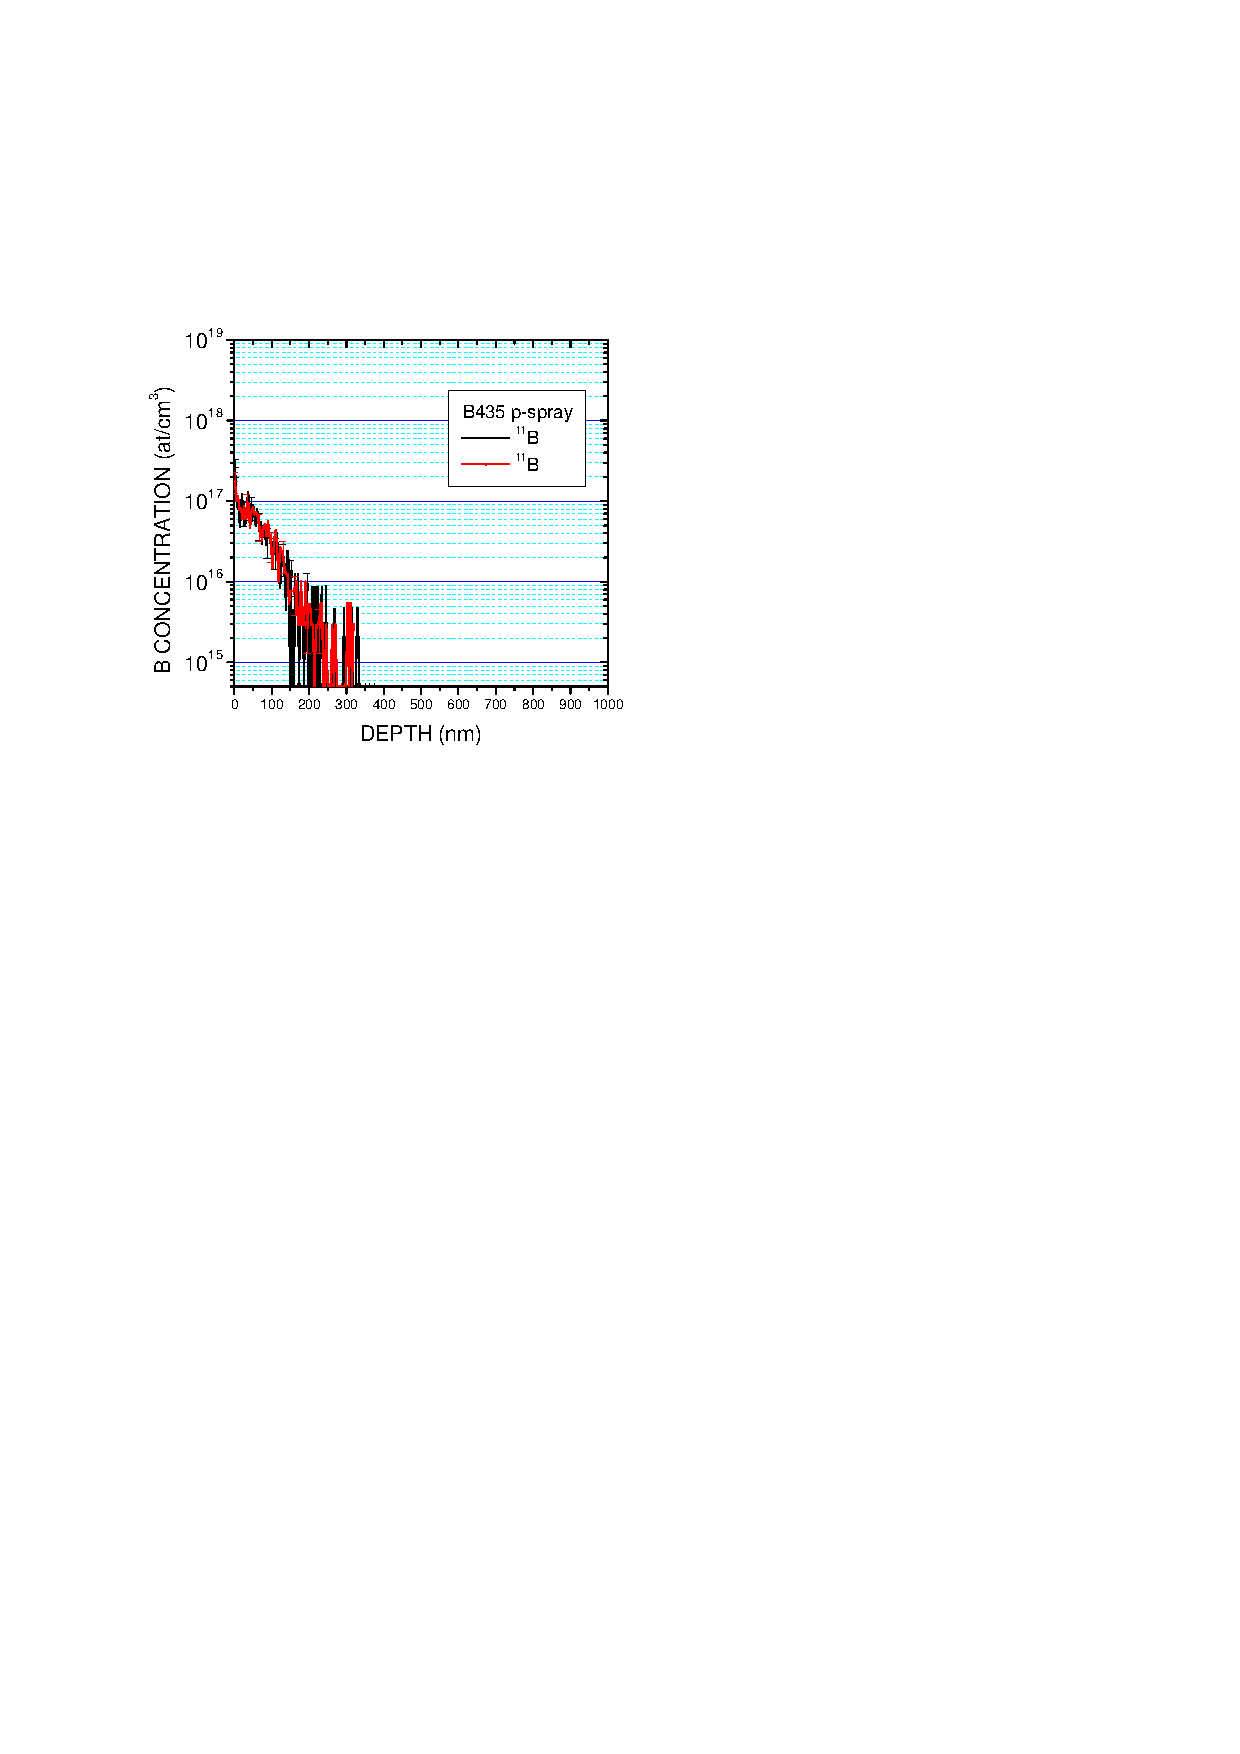
\includegraphics[width=0.65\textwidth]{sims_pspray.pdf}
\caption{\label{fig:sims_pspray}Boron depth profiles obtained in two points for each {\it p-spray} area 
on samples taken from an $n-on-p$ production.}
\end{figure}

P-spray is needed to counter the accumulation of electrons between $n^+$ implants in an 
electron collecting detector, which otherwise would short the electrodes and degrade the 
detector performance. The positive oxide charge is the responsible for the electron layer 
at the Si-SiO$_2$ interface~\cite{Lutz:411172}. 

Thanks to inputs like the ones from SIMS it is possible to make optimal choices for the detector 
edge design as it was done for the edgeless pixels sensors reported in~\cite{bib:nim2012}. 
An example of the agreement between real data and TCAD simulations is shown in 
Figure~\ref{fig:IV_BD}.
\begin{figure}[!htbp]
\centering
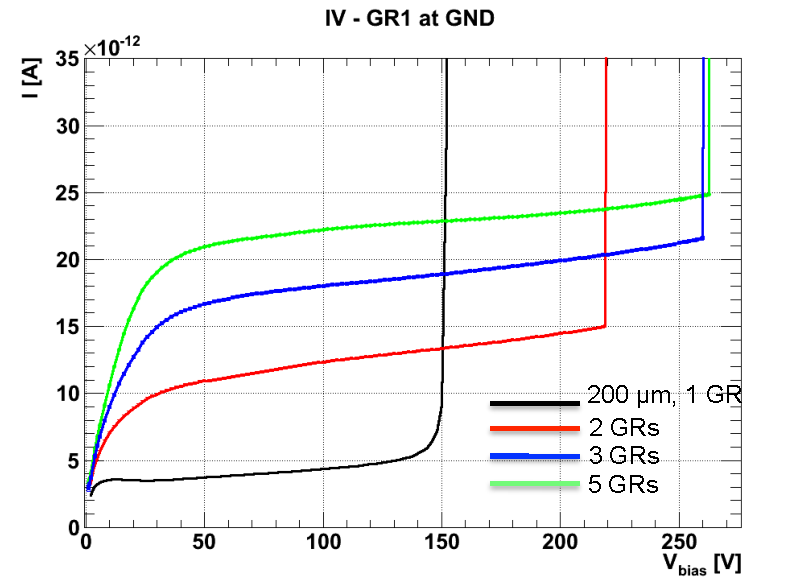
\includegraphics[width=0.5\textwidth]{IV_simulations}
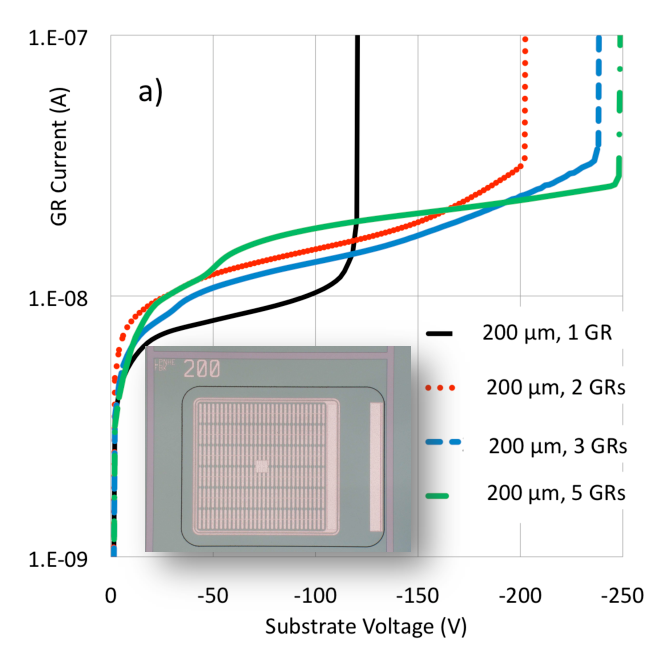
\includegraphics[width=0.39\textwidth]{IV_data}
\caption{\label{fig:IV_BD}IV curves for edgeless $n-on-p$ pixel test structures. (left) TCAD simulations 
(right) Real data from~\cite{bib:nim2012}. Detectors with the same pixel-to-edge minimal distance 
and different number of GRs are compared. In the right figure a photo of the tested detector is 
shown in the inset.}
\end{figure}
In the Figure the IV curves of edgeless $n-on-p$ pixel test structures are compared. The 
parameter of interest here is the breakdown (BD) voltage, which in the presence of 
p-spray depends critically on the dose of the implant and on the shape of the electrode 
on top of the $n^+$ implant. 

As it can be seen for what concerns the BD voltage the level of agreement between real data 
and TCAD simulations is at 20\% or better. This was an important achievement since 
the designs of the real sensors was driven by the TCAD simulations studies; they allowed 
to choose among different possible combinations of minimal pixel-to-edge distances and 
number of GRs. 

A similar studied, reported in Figure~\ref{fig:width_GRs}, showed that keeping the number of GRs fixed and simply increasing the 
minimal pixel-to-edge distance doesn't make the BD voltage larger.

\begin{figure}[!htbp]
\centering
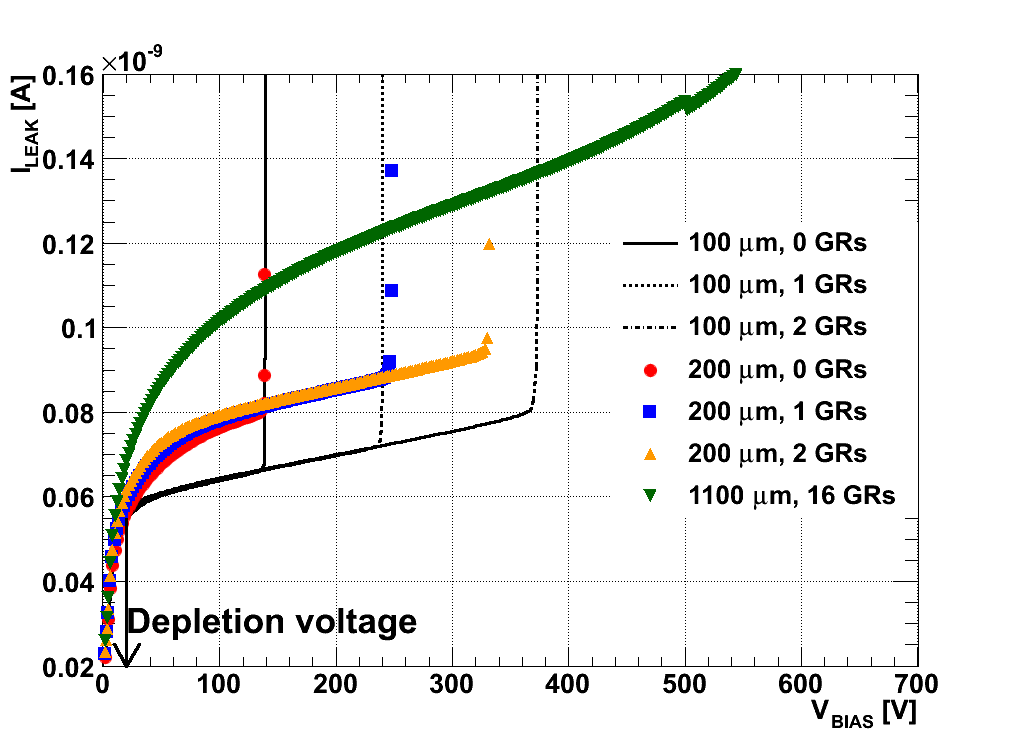
\includegraphics[width=0.65\textwidth]{edgeless_BD_FL0_BandW_mix}
\caption{\label{fig:width_GRs}Simulated IV curves for edgeless $n-on-p$ pixel test structures. Detectors with different pixel-to-edge minimal distance 
and different number of GRs are compared.}
\end{figure}

This effect is due to the p-spray which is equipotential till it doesn't cross a $n^+$ implant, like a 
GR or the pixels. Hence, increasing the distance between the detector edge and the pixels but 
not adding more GRs doesn't allow a more smooth voltage drop, hence doesn't change the 
BD voltage. The fact the p-spray is equipotential was verified during the simulation studies, a test 
otherwise difficult to accomplish.


The one presented so far is a very simple but effective case in which TCAD simulations drive the 
sensors design. More sophisticated studies can be carried out, in which processes like 
etching, oxide growing, doping implantation and diffusion and many more can be simulated. 
These kind of studies are beyond the scope of this report; an example of such studies 
can be found in~\cite{CISSIMDET2014}. 

\section{Sensor Simulation}
\label{sec:sensorsimulation}

Sensor simulation allows to study the detector behaviour under numerous conditions like 
forward~/~reverse voltage, application of sinusoidal signals on electrodes, illumination with lasers or 
generally light, generation of charge in the 
bulk by charged particles, radiation induced traps in the bulk and at the surface, low temperature 
operation, etc., 
and of course combination of them.
All these correspond to working condition for HEP detectors, hence predictions can be extracted 
for example for a heavily irradiated silicon detector in terms of charge collection efficiency, operating 
voltage and leakage current level.

Again such studies allow to make detector choices that save money and time and give access to 
quantities like carriers distribution otherwise impossible to measure. An example is given in 
Figure~\ref{fig:carr_conc}, where the result of 2D simulations of an  $n-on-p$ detector 
are reported.

\begin{figure}[!htbp]
\centering
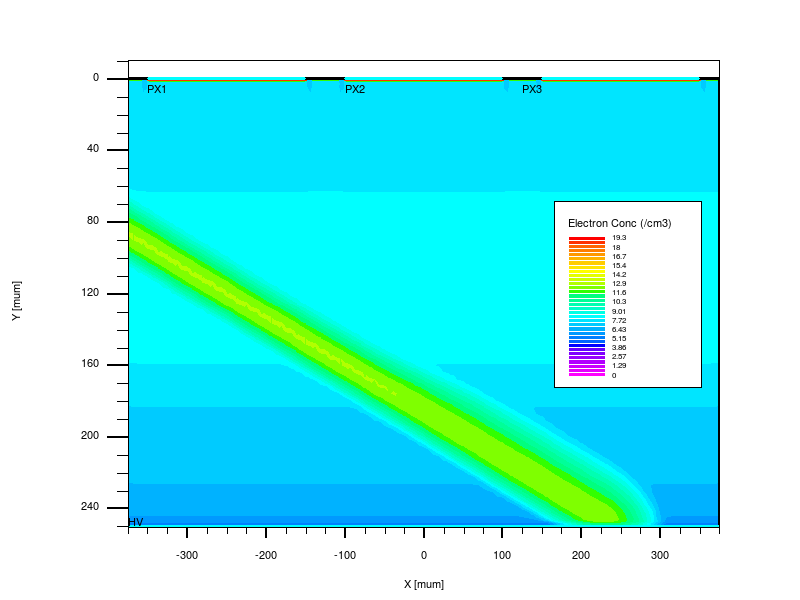
\includegraphics[width=0.45\textwidth]{econ_early.png}
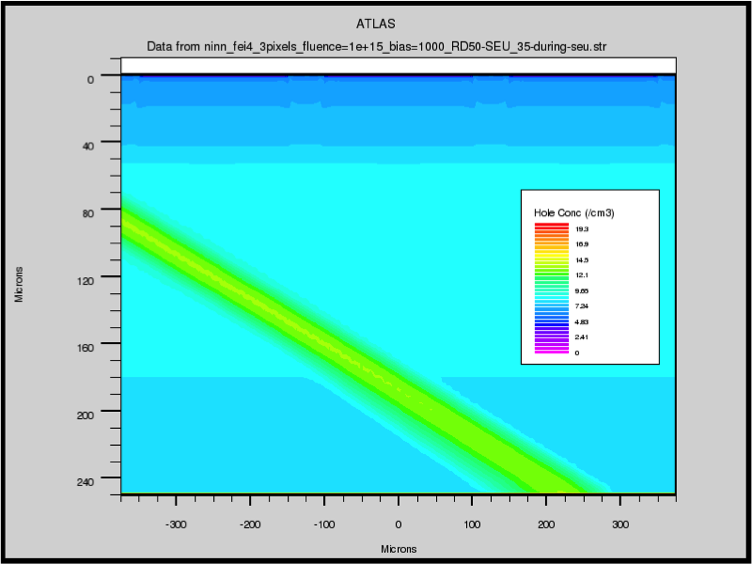
\includegraphics[width=0.45\textwidth]{hcon_early.png}
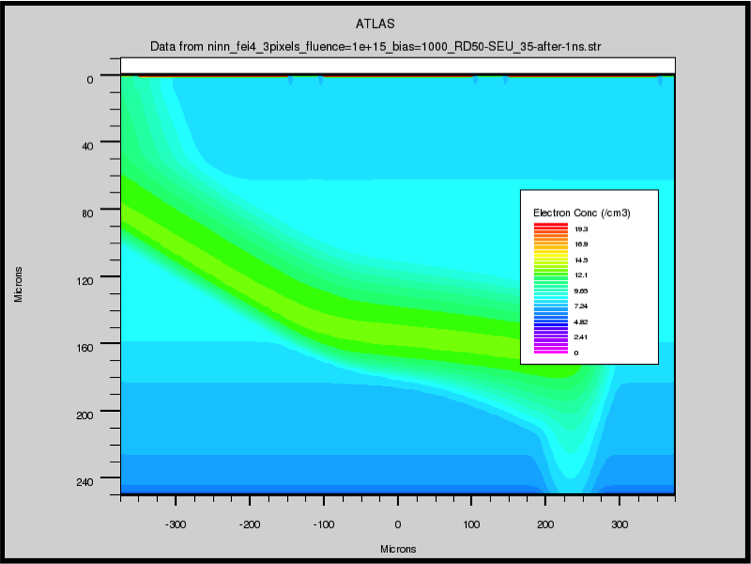
\includegraphics[width=0.45\textwidth]{econ_late.png}
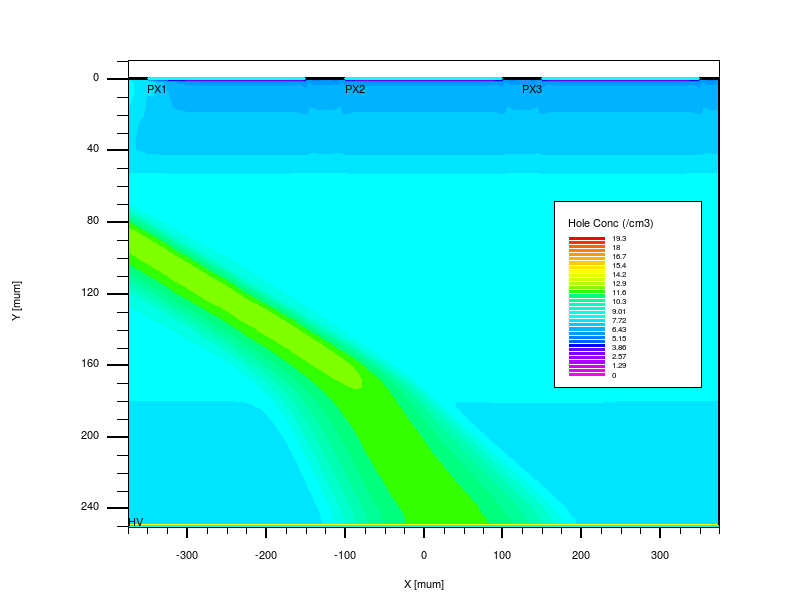
\includegraphics[width=0.45\textwidth]{hcon_late.png}
\caption{\label{fig:carr_conc}2D simulations of an $n-on-p$ detector. Carriers concentration
are reported when the detector is over depleted and a MIP stroke at $t=0$~s. 
(Top) Carriers distribution during the MIP strike. (Bottom) After 1~ns. (Left) electron concentration. 
(Right) Hole concentration. MIP was impinging at 20$^{\circ}$ with respect to the sensor surface.}
\end{figure}

Three collecting electrodes are simulated; the detector is 250~$\mu$m thick and the pitch 
is 250~$\mu$m. The detector is hit my a MIP when it is in over-depletion; the MIP strikes at 
an angle of 20$^{\circ}$ with respect to the sensor surface. The detector was simulated after 
an irradiation fluence of $\Phi=1\times10^{15}$~n$_{\rm eq}$/cm$^2$
It can be seen from the Figure that electrons drift faster than holes; a large fraction of holes 
have moved little from the original position while electrons have gained much more distance 
after 1~ns. 

This kind of simulation are needed to interpret data from test beams when tracks are impinging 
at shallow angle. The charge profile in data can be compared over the signal amplitude from pixels in 
long clusters to the one predicted by TCAD simulations; this will allow to infer the electric field 
distribution inside the irradiated detector thanks to so-called {\it grazing angle} 
technique~\cite{Henrich:687041,Lari:2001qqa}; more 
on this in the next Section.

In case of edgeless sensors it is interesting to investigate the charge collection efficiency (CCE) 
in the un-instrumented area between the last collecting electrode and the detector edge. 
Other than the BD voltage, also CCE is an important factor on which optimise the 
detector design. In Figure~\ref{fig:Edgeless_CCE} the result of a simulation study for an 
$n-on-p$ edgeless detector 
\begin{figure}[!htbp]
\centering
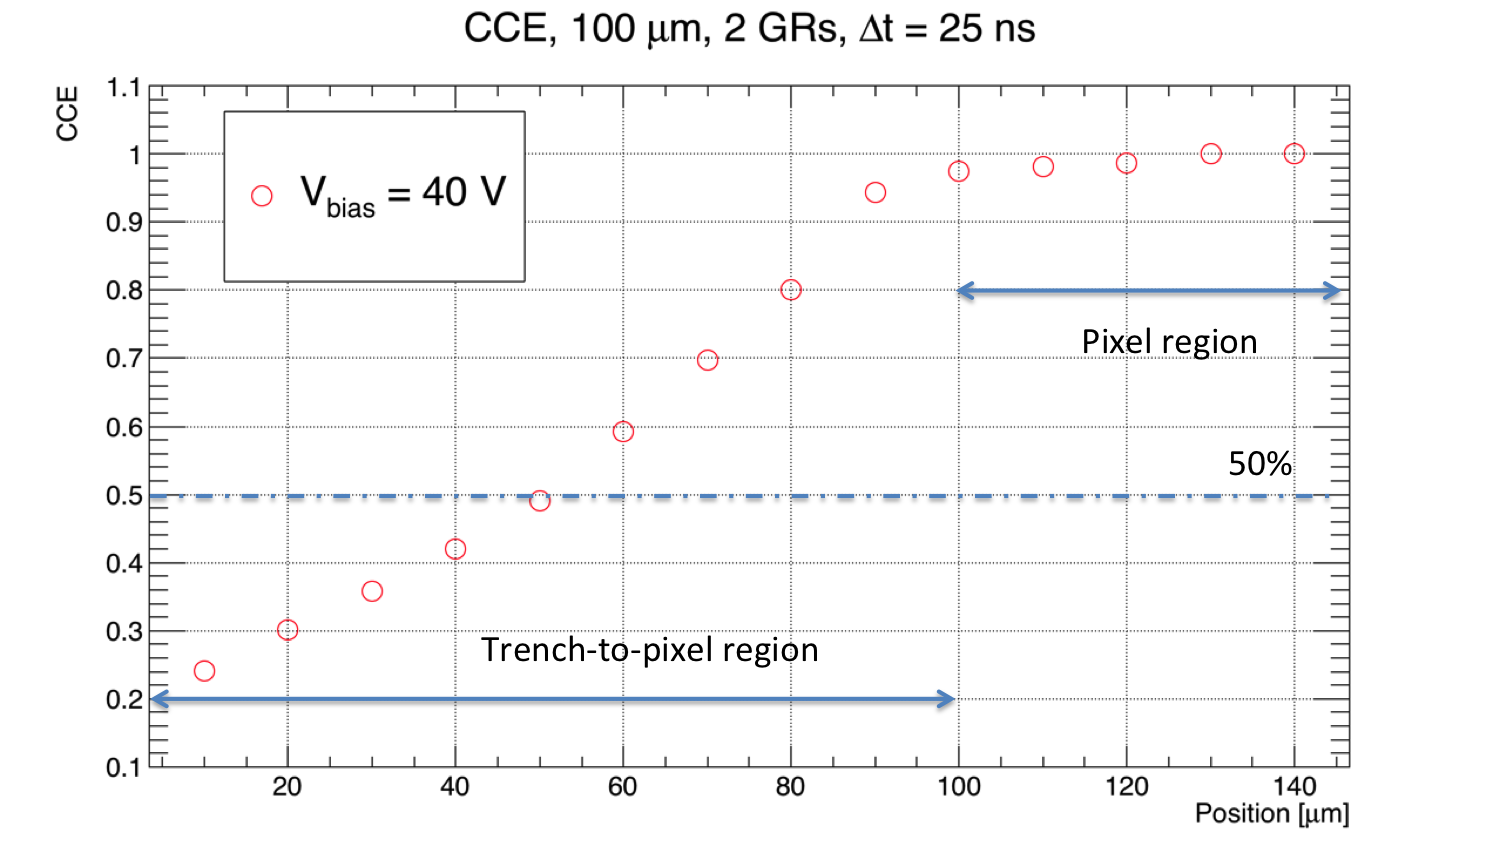
\includegraphics[width=0.65\textwidth]{Edgeless_CCE.png}
\caption{\label{fig:Edgeless_CCE}Simulated CCE as a function of the MIP impact point. 
It is the result of a 2D simulations of an $n-on-p$ edgeless detector. The bias voltage and the integration time 
are indicated.}
\end{figure}

The simulations indicate that it is possible to collect at least 50\% of the signal amplitude for a MIP 
up to 50~$\mu$m away from the last collecting electrode. This is very promising for {\it active edge} 
detectors  (see also~\ref{sec:edgeless}).

\section{Discussion on Fundamental Parameters and TCAD Simulations}
The two most used commercial TCAD products in the HEP community are Silvaco\footnote{\url{https://www.silvaco.com/products/tcad.html}} and Synopsys\footnote{\url{https://www.synopsys.com/silicon/tcad.html}}.

In a test to see how much the two products differ in terms of physics models it turned out 
that at least in two fundamental semiconductor physics observables they were quite far apart. 
The result of the investigations are documented in~\cite{bomben_rd50_Torino}.

The first observable under investigation was the thermal velocities of the carriers. The results 
are illustrated in Figure~\ref{fig:vtherm}.

\begin{figure}[!htbp]
\centering
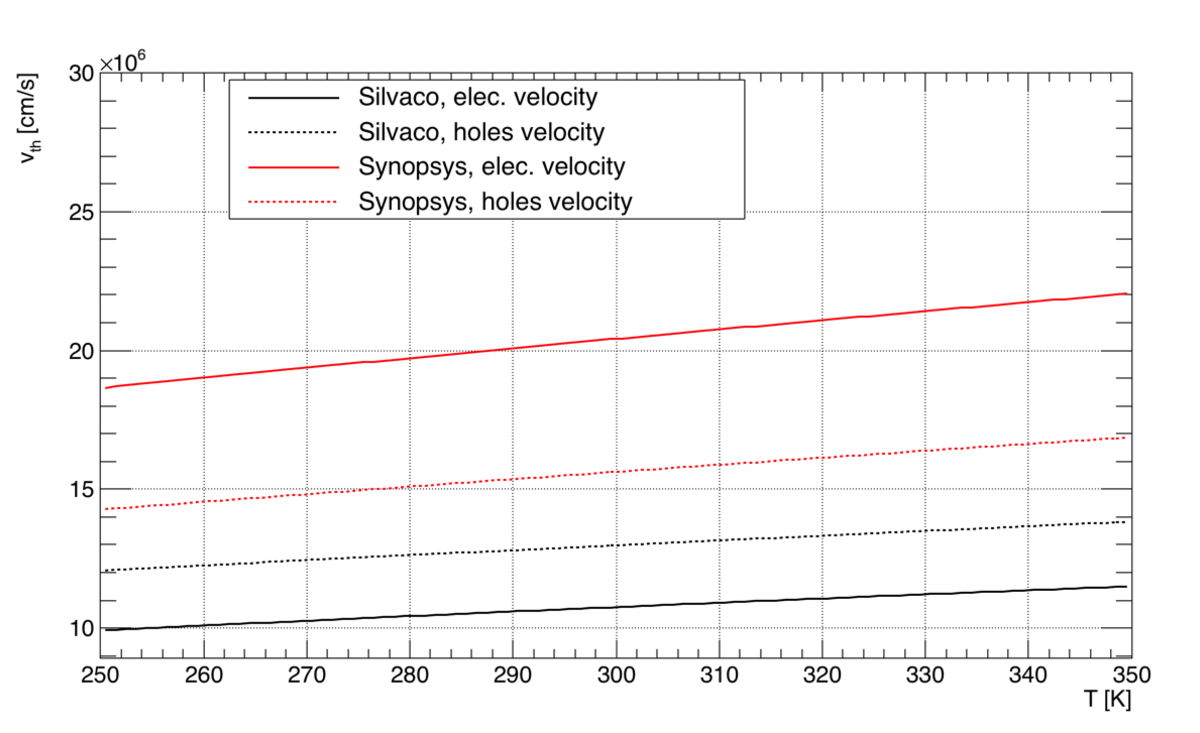
\includegraphics[width=0.65\textwidth]{vtherm}
\caption{\label{fig:vtherm}Carrier thermal velocities as a function of the temperature.}
\end{figure}
As it can be seen there is almost a factor of 2 of difference between the two tools for the electrons 
thermal velocities. The reason for this disagreement has to be found in the carriers  mass value
used in the thermal velocities calculation. While Synopsys uses the effective  mass derived 
from the energy band curvature, Silvaco inserts the rest mass of the electron. 
Such a difference in the  carriers thermal velocities affect the carriers transport phenomena, 
the leakage current level and the effects due to radiation damage defects. 
 
 The second parameter that was investigated was the bandgap energy $E_g$. The default value in 
 Silvaco for $E_g$ at $T=$300~K is of 1.08~eV. This is surprisingly low compared to values in literature 
 (see for example~\cite{Lutz:411172,Sze1981,Wang1989,Shockley}) which are comprised 
 in the range 1.11-1.12~eV.
The temperature dependence of $E_g$ is based on~\cite{Sze1981}:
\begin{equation}
E_g(T)=E_g(0) -\dfrac{\alpha T^2}{T+\beta}=E_g(300)+\alpha\Bigg[ \dfrac{(300)^2}{300+\beta}-\dfrac{T^2}{T+\beta}  \Bigg] \equiv E_g(T_{ref})+\alpha\Bigg[ \dfrac{(T_{ref})^2}{T_{ref}+\beta}-\dfrac{T^2}{T+\beta}  \Bigg] 
\label{eq:EgT}
\end{equation}
where $T_{ref}$ is some reference temperature.
Both TCAD products agree on the $\alpha$ and $\beta$ parameters values:

\begin{table}[!htbp]
\caption{\label{eq:Egalphabeta}Parameter values for the temperature dependence of the bandgap. 
See also Equation~\ref{eq:EgT}}
\centering
\begin{tabular}{|c|c|}
\hline
parameter & value \\
\hline 
$\alpha$ & 4.73$\times$10$^{-4}$~eV/K \\
\hline 
$\beta$ & 636~K \\
\hline
\end{tabular}
\end{table}

Silvaco tools are built on the value $E^{Sil}_g(300)=$1.08~eV while Synopsys on $E^{Syn}_g(0)=$1.1696~eV. 
Extrapolating $E_g^{Syn}(0)$ to $T=$300K from the one gets the expected 
$E_g^{Syn}(300)\sim$1.12~eV, in agreement with literature.

Silvaco developers explained\footnote{private communication} the abnormal $E^{Sil}_g(300)$ value 
because of very low resistivity 
Silicon wafers used to estimate the bandgap energy when their TCAD tool was developed. 
They are aware of the issue and claim that the Silvaco TCAD tools are anyhow consistent with 
the $E^{Sil}_g(300)$ value chosen and predictions are reliable. The 

To test the latter statement the $E^{Sil}_g(300)$ value was changed in the simulation package, 
and results compared. 
A 200~$\mu$m thick, 50~$\mu$m wide $n-on-p$ diode was simulated using Silvaco 2D device 
simulator. Temperature was varied between -20$^{\circ}$ and +20$^{\circ}$ in 5$^{\circ}$ steps. 
Several scenarios have been invetigated:

\begin{itemize}
\item[\bf default] using default Silvaco parameters values
\item[\bf EG112] setting $E^{Sil}_g(300)=1.12$~eV
\item[\bf Syn. Th. Vel.] setting thermal velocities to the values used by Synopsys tool
\item[\bf EG112 \& Syn. Th. Vel.] combination of the two above 
\item[\bf NO BGN] turning off the model for bandgap narrowing based on the concentrations~\cite{SLOTBOOM1977279}.
\end{itemize}

Several studies were performed using the Silvaco TCAD tools,
 including comparison of simulated leakage current level with 
theoretical expectations,  evaluation of the activation energy $E_{a}$ (Equation~\ref{eq:IleakT}) 
and scaling of leakage current with temperature. In what follows the findings of these 
studies and the discussion.

\subsubsection{Leakage Current Level}




In Figure~\ref{fig:ILeak20C} a comparison of the simulated leakage current in the five scenarios for $t=20^{\circ}$C is presented.
\begin{figure}[!htbp]
\centering
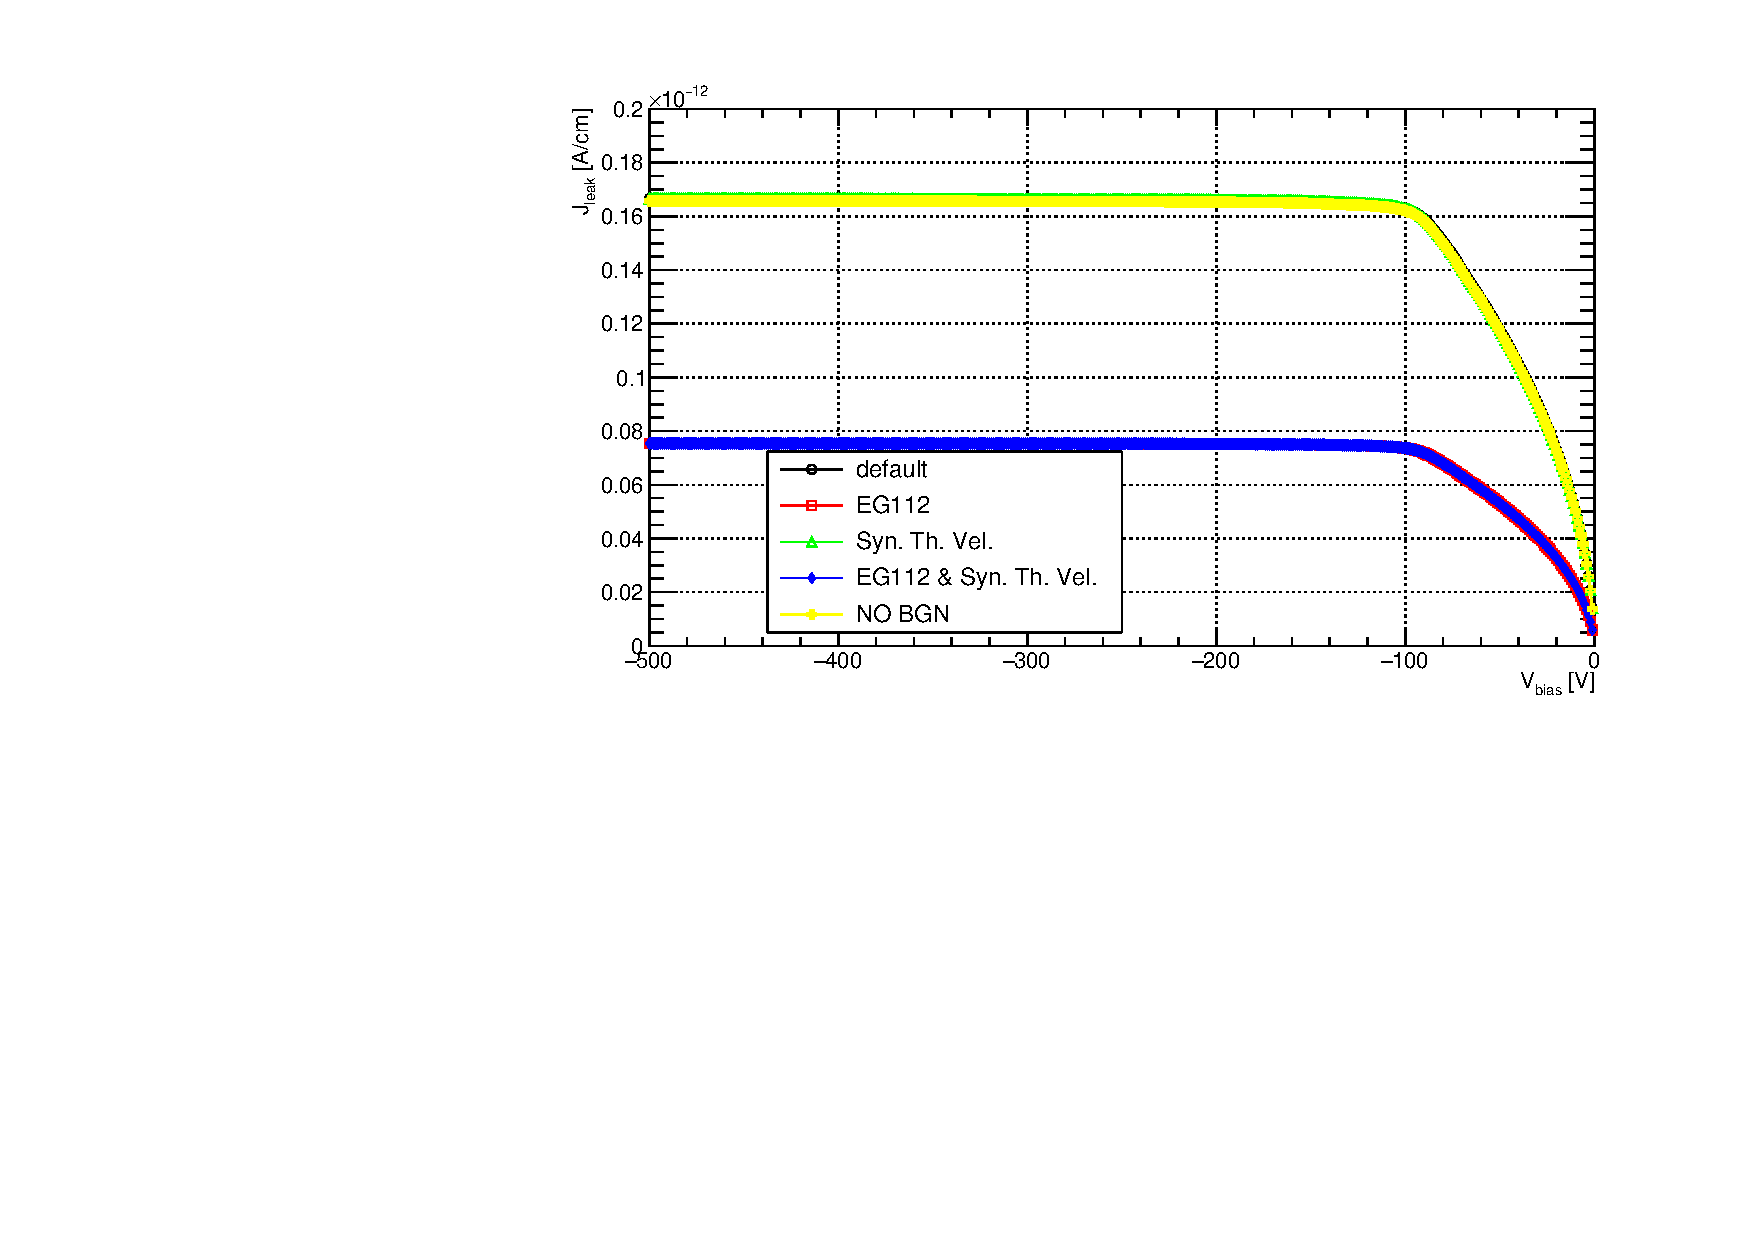
\includegraphics[width=0.65\textwidth]{currents_T20_scenarios.pdf}
\caption{\label{fig:ILeak20C}Simulated current density as a function of the bias voltage for different 
scenarios at $t=20^{\circ}$C. See text for more details.}
\end{figure}
It is evident that the only parameter playing a major role, as expected, is the bandgap energy $E^{Sil}_g(300)$. 



To verify the validity of leakage current level  from Silvaco tools the result at $V_{op}$ bias 
were compared with the theoretical value evaluated using~\ref{eq:Ileak2}. Assuming the same value
for generation and recombination lifetimes and taking the intrinsic concentration value $n_i$ from 
the simulation itself a current density of $J\sim1.6\times10^{-13}$~A/cm is expected, which 
is in excellent agreement with the value observed in simulations when the default value of 
$E^{Sil}_g(300)$ is chose ({\it i.e.} 1.08~eV); on the contrary, as it can be seen from Figure~\ref{fig:ILeak20C}, when $E^{Sil}_g(300)$ is set to 1.12~eV the simulation results don't match 
the theoretical expected values.

It has to be noted that  the simulated current is purely bulk generated; this is also clear from 
Figure~\ref{fig:ILeak20C}: the current level is stable after the depletion voltage. This feature 
is not realistic~\cite{CALZOLARI19721003} but for the sake of understating bulk generated 
current properties in TCAD simulations is very well suited since it allows to study the 
phenomenon without having to deconvolve from the current surface effects, trap assisted tunnelling 
and others.

\subsubsection{Temperature Dependence of Simulated Leakage Current and Activation Energy}

The change of leakage current was studied for the different scenarios outlined before. 
For all temperature $T$ times scenario $S$ combination the leakage current $I_{leak}(V_{op};T;S)$ 
at a 
operational voltage 
$V_{op}$ defined as:

\begin{equation}
V_{op}=V_{depl}+50\,{\rm V}
\label{eq:Vop}
\end{equation} 
was extracted. It was verified that the depletion voltage $V_{depl}$ didn't depend on scenarios nor temperatures.

 The leakage current was then studied as a function of the reciprocal of the 
temperature and fitted with a function inspired by Equation~\ref{eq:IleakT}:

\begin{equation}
I = I_{ref}\Bigg(\dfrac{T}{T_{ref}}\Bigg)^n exp^{\Bigg[ -\dfrac{E_{a}}{2k_B}\Bigg( \dfrac{1}{T}- \dfrac{1}{T_{ref}} \Bigg) \Bigg]}
\label{eq:ITfunc}
\end{equation}
where $n$ and $E_{a}$ are free parameters, $I_{ref}$ the simulated current at the reference 
temperature $T_{ref}$ and $k_B$ the Boltzmann constant.
The results are reported in Figure~\ref{fig:Ea_Fit}. A 0.01~K error was assigned to the 
simulated temperature, the leakage current was evaluated at $V_{op}\pm1.0$~V too and the largest 
shift used as an uncertainty estimate.
In Figure~\ref{fig:Ea_Fit_fixn} the  parameter $n$ was fixed to 2.

\begin{figure}[!htbp]
\centering
\includegraphics[width=0.49\textwidth]{default/Ea_Fit.pdf}\\
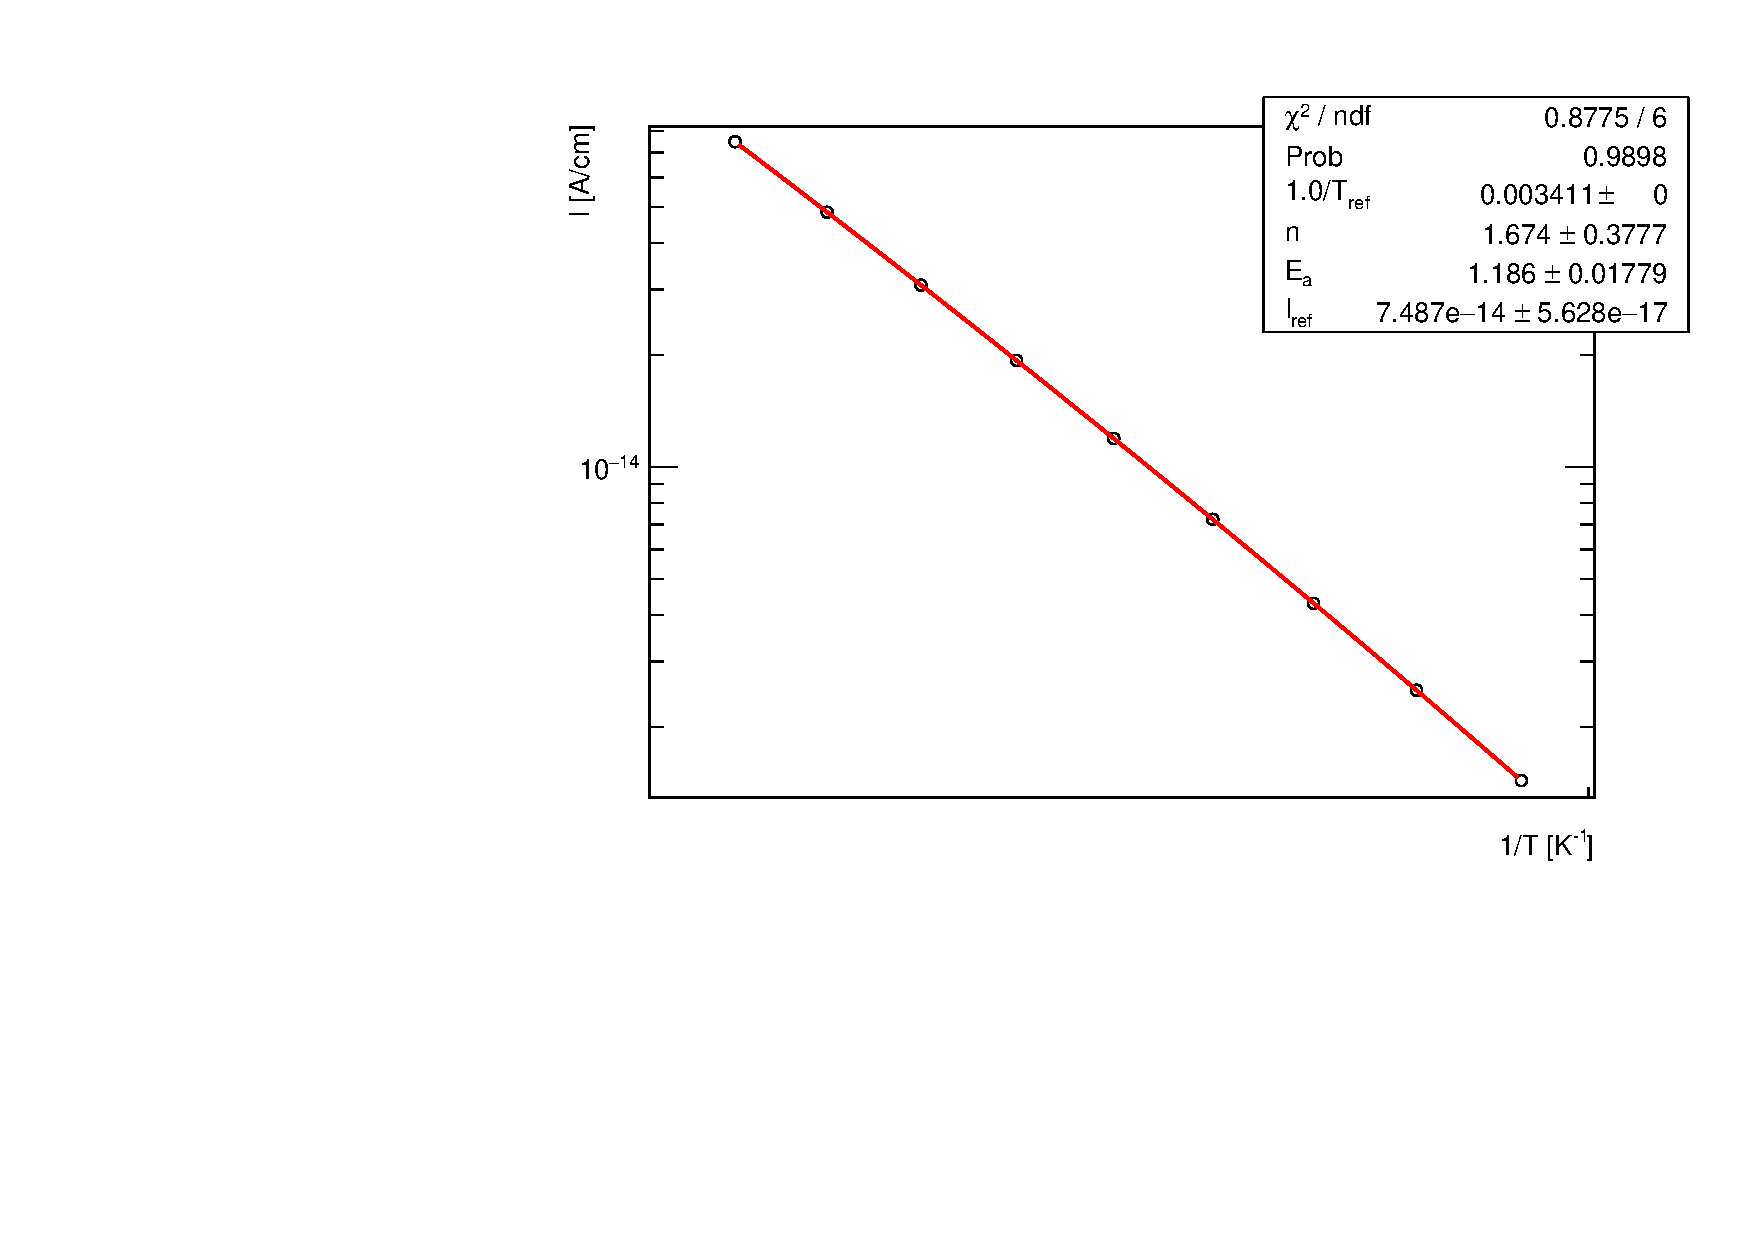
\includegraphics[width=0.49\textwidth]{EG112/Ea_Fit.pdf}
\includegraphics[width=0.49\textwidth]{Syopsys_thermal_velocities/Ea_Fit.pdf}
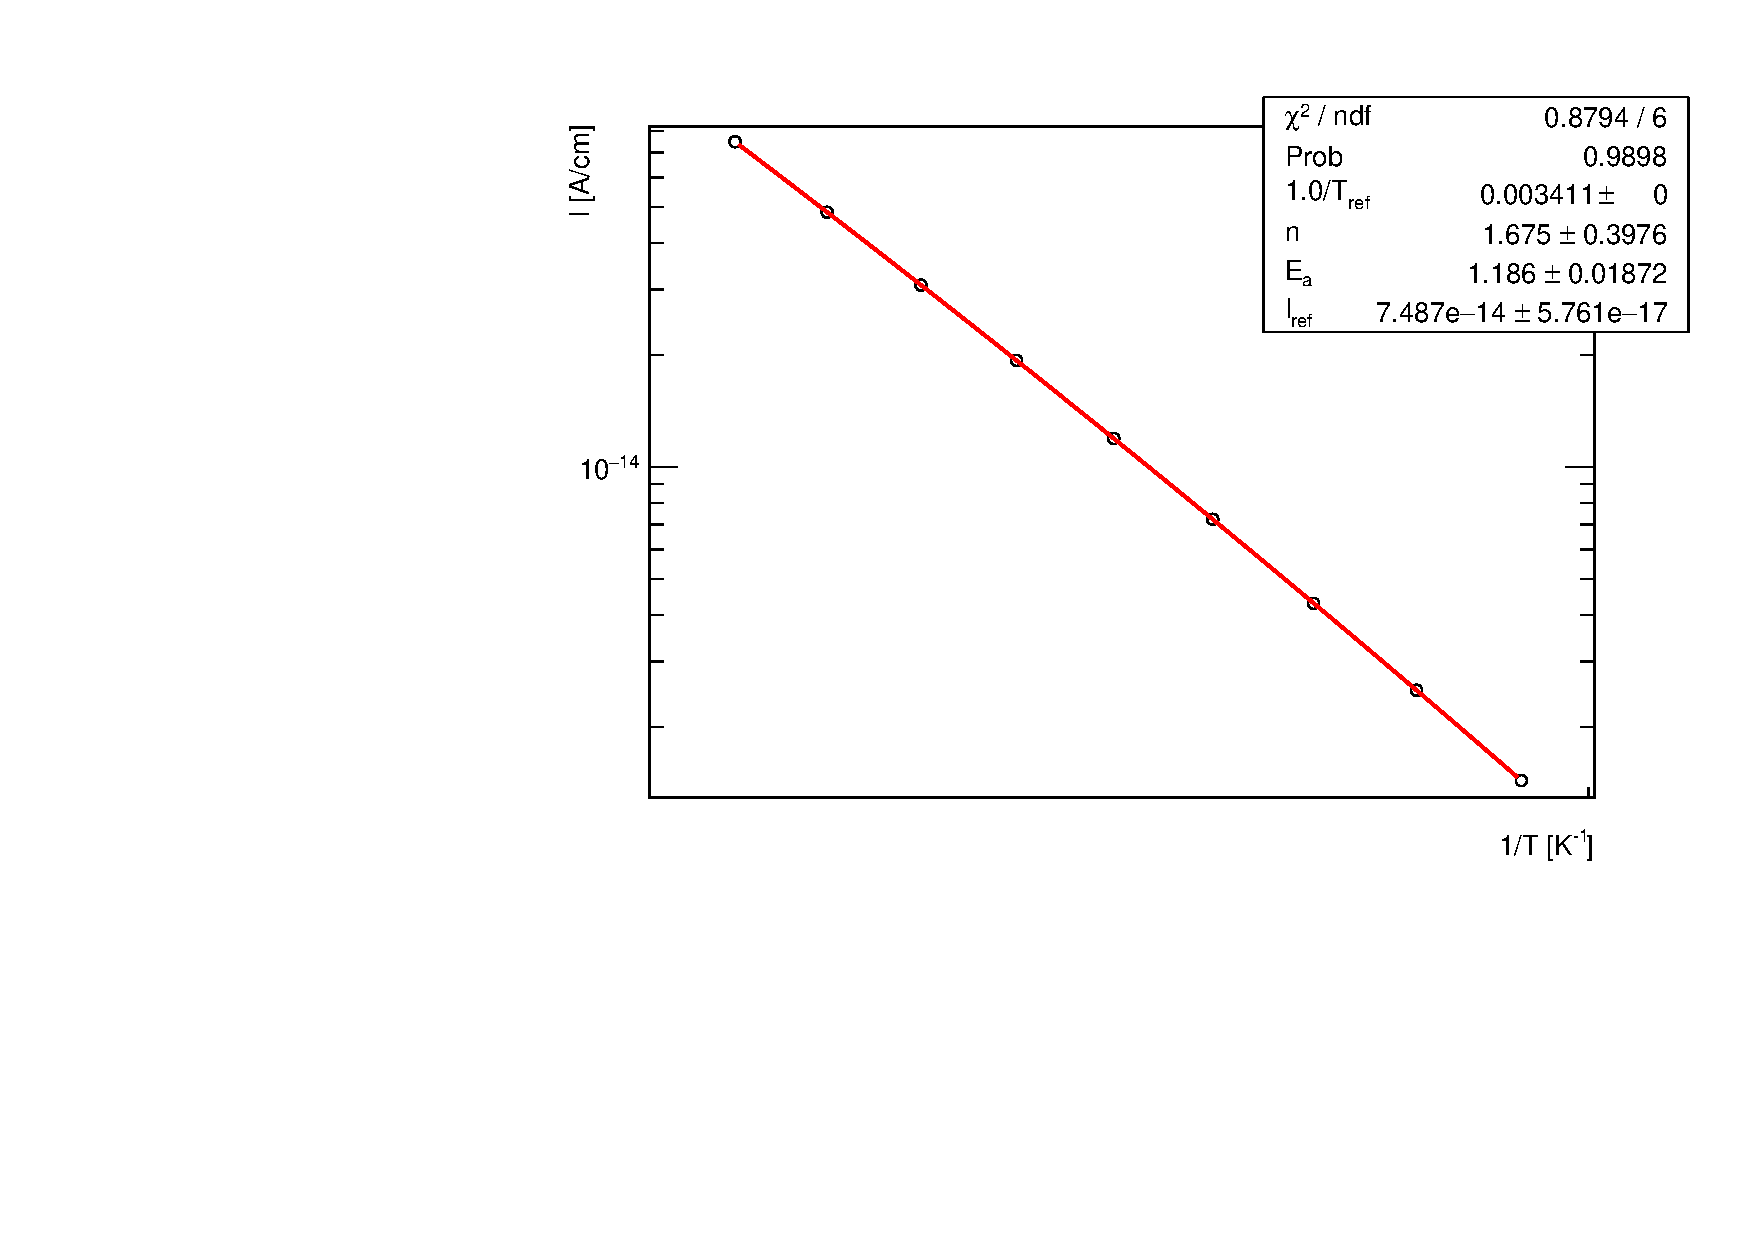
\includegraphics[width=0.49\textwidth]{EG112_Syopsys_thermal_velocities/Ea_Fit.pdf}
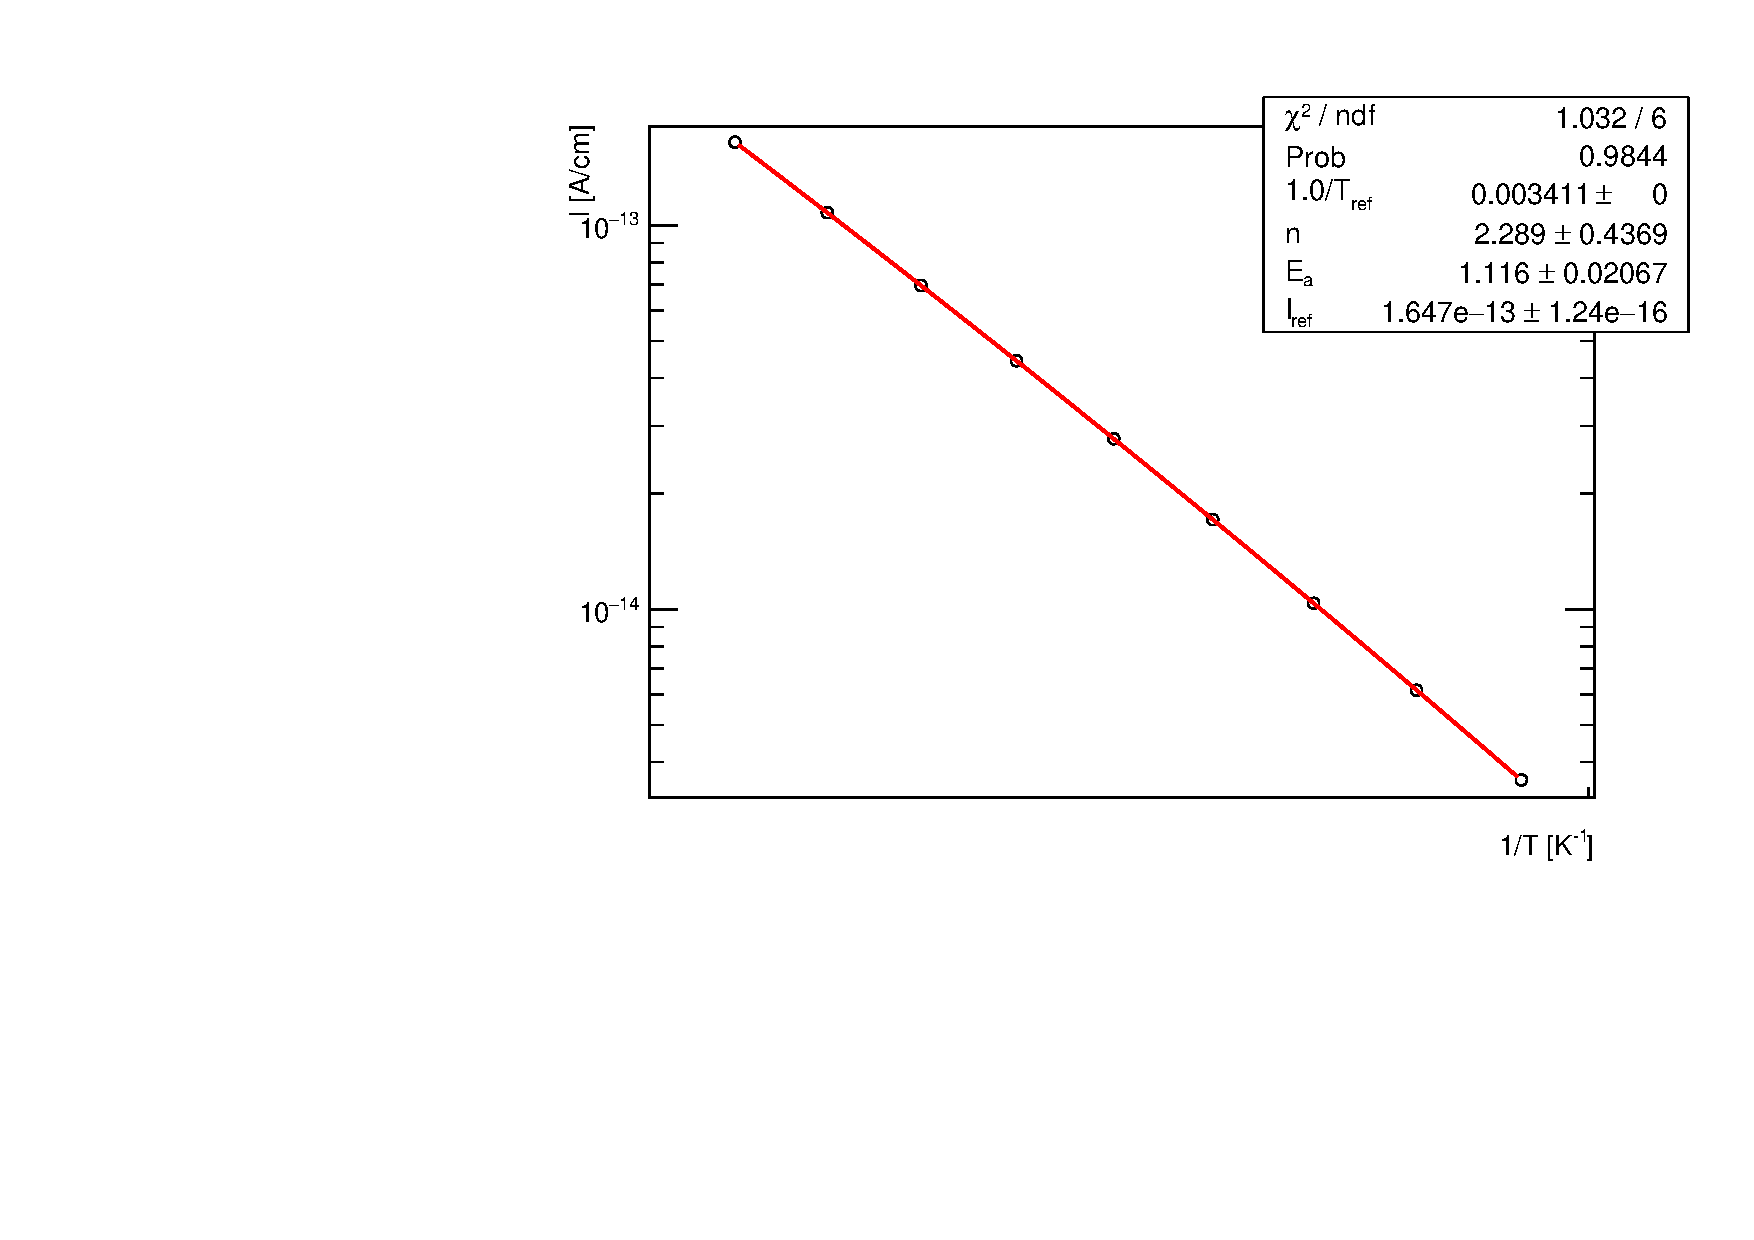
\includegraphics[width=0.49\textwidth]{nobgn/Ea_Fit.pdf}
\caption{\label{fig:Ea_Fit}. Simulated leakage current at operational voltage $V_{op}$ at different 
temperatures for different scenarios. (Top row) default scenario; (mid row) EG112 scenario on the left,  Syn. Th. Vel. on the right;  (bottom row)  EG112 \&  Syn. Th. Vel. scenario on the left, NO BGN 
on the right. Data are points with error bars; data were fit with Equation~\ref{eq:ITfunc}  and the fit result is superimposed.}
\end{figure}


\begin{figure}[!htbp]
\centering
\includegraphics[width=0.49\textwidth]{default/Ea_Fit_fixn.pdf}\\
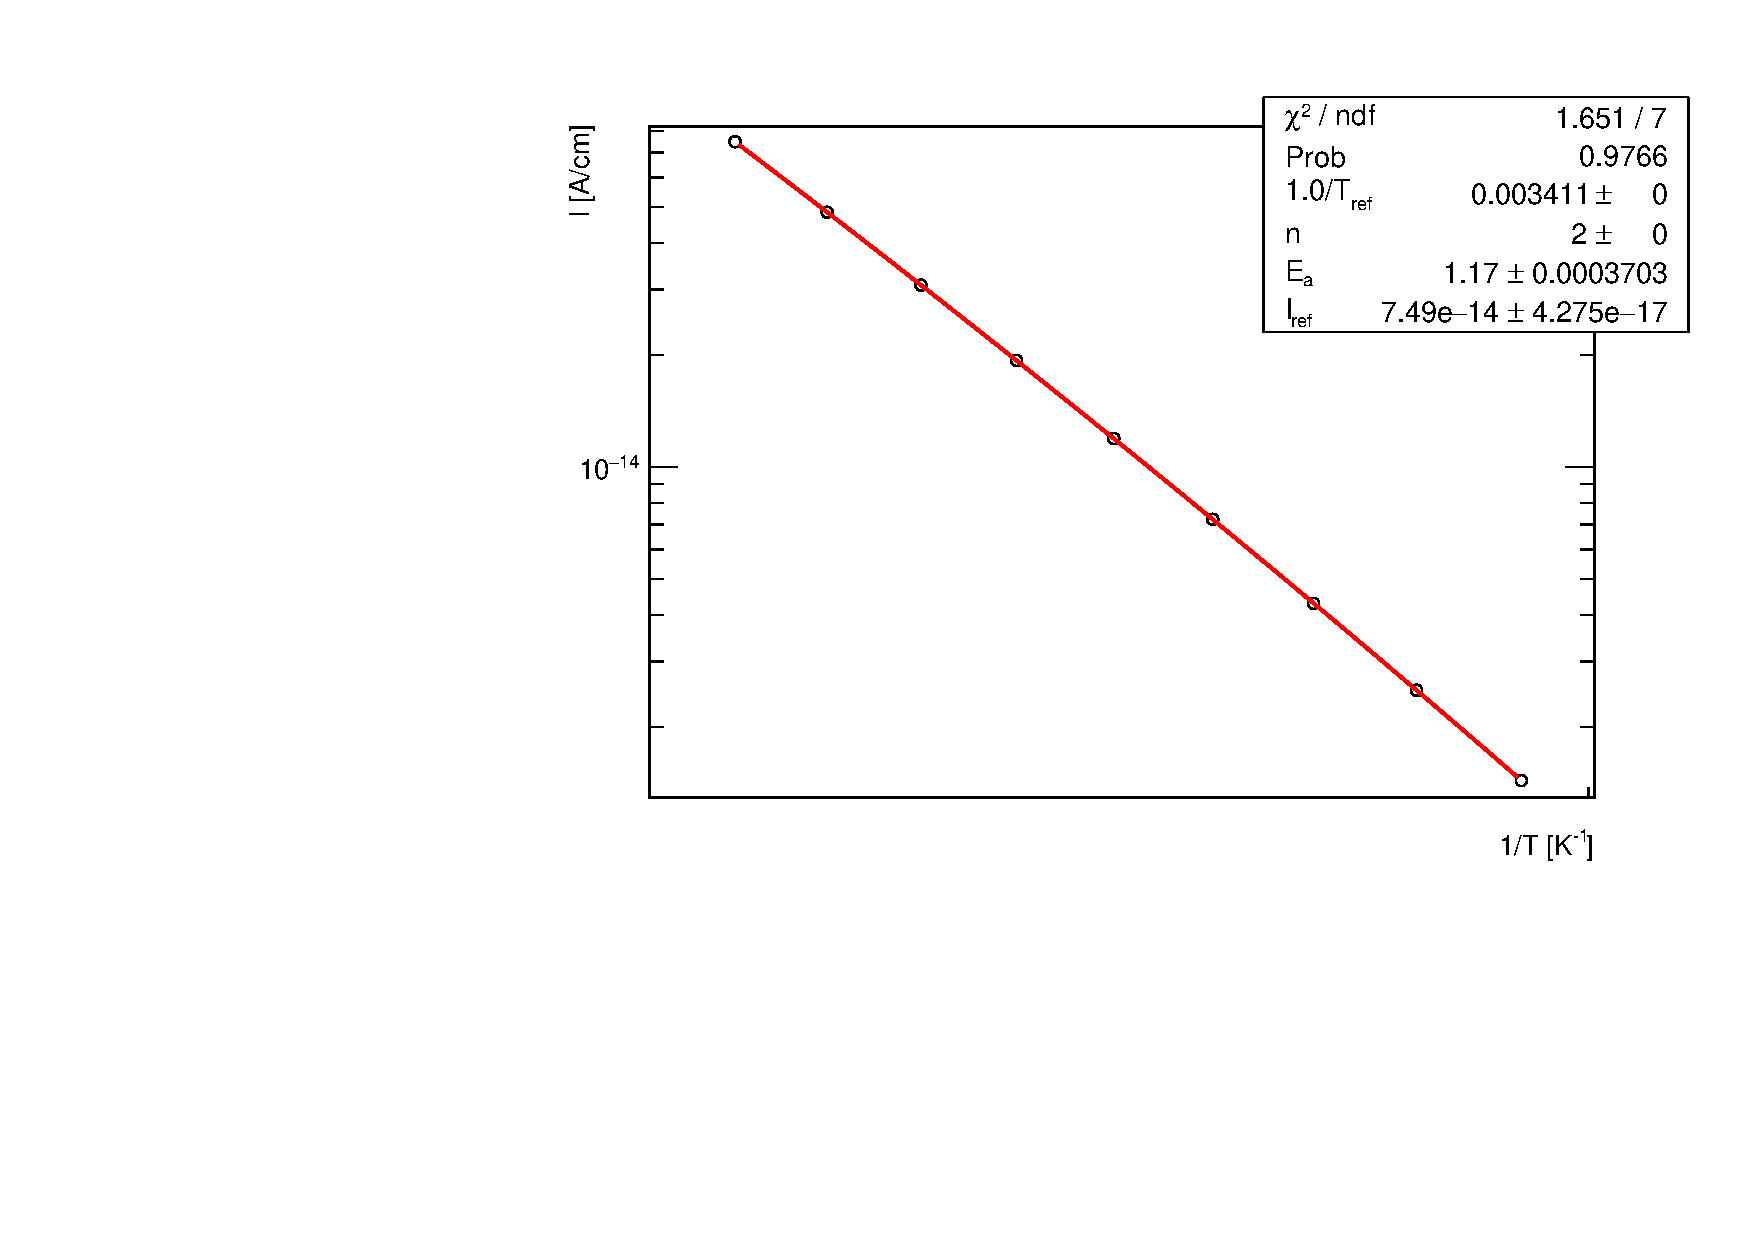
\includegraphics[width=0.49\textwidth]{EG112/Ea_Fit_fixn.pdf}
\includegraphics[width=0.49\textwidth]{Syopsys_thermal_velocities/Ea_Fit_fixn.pdf}
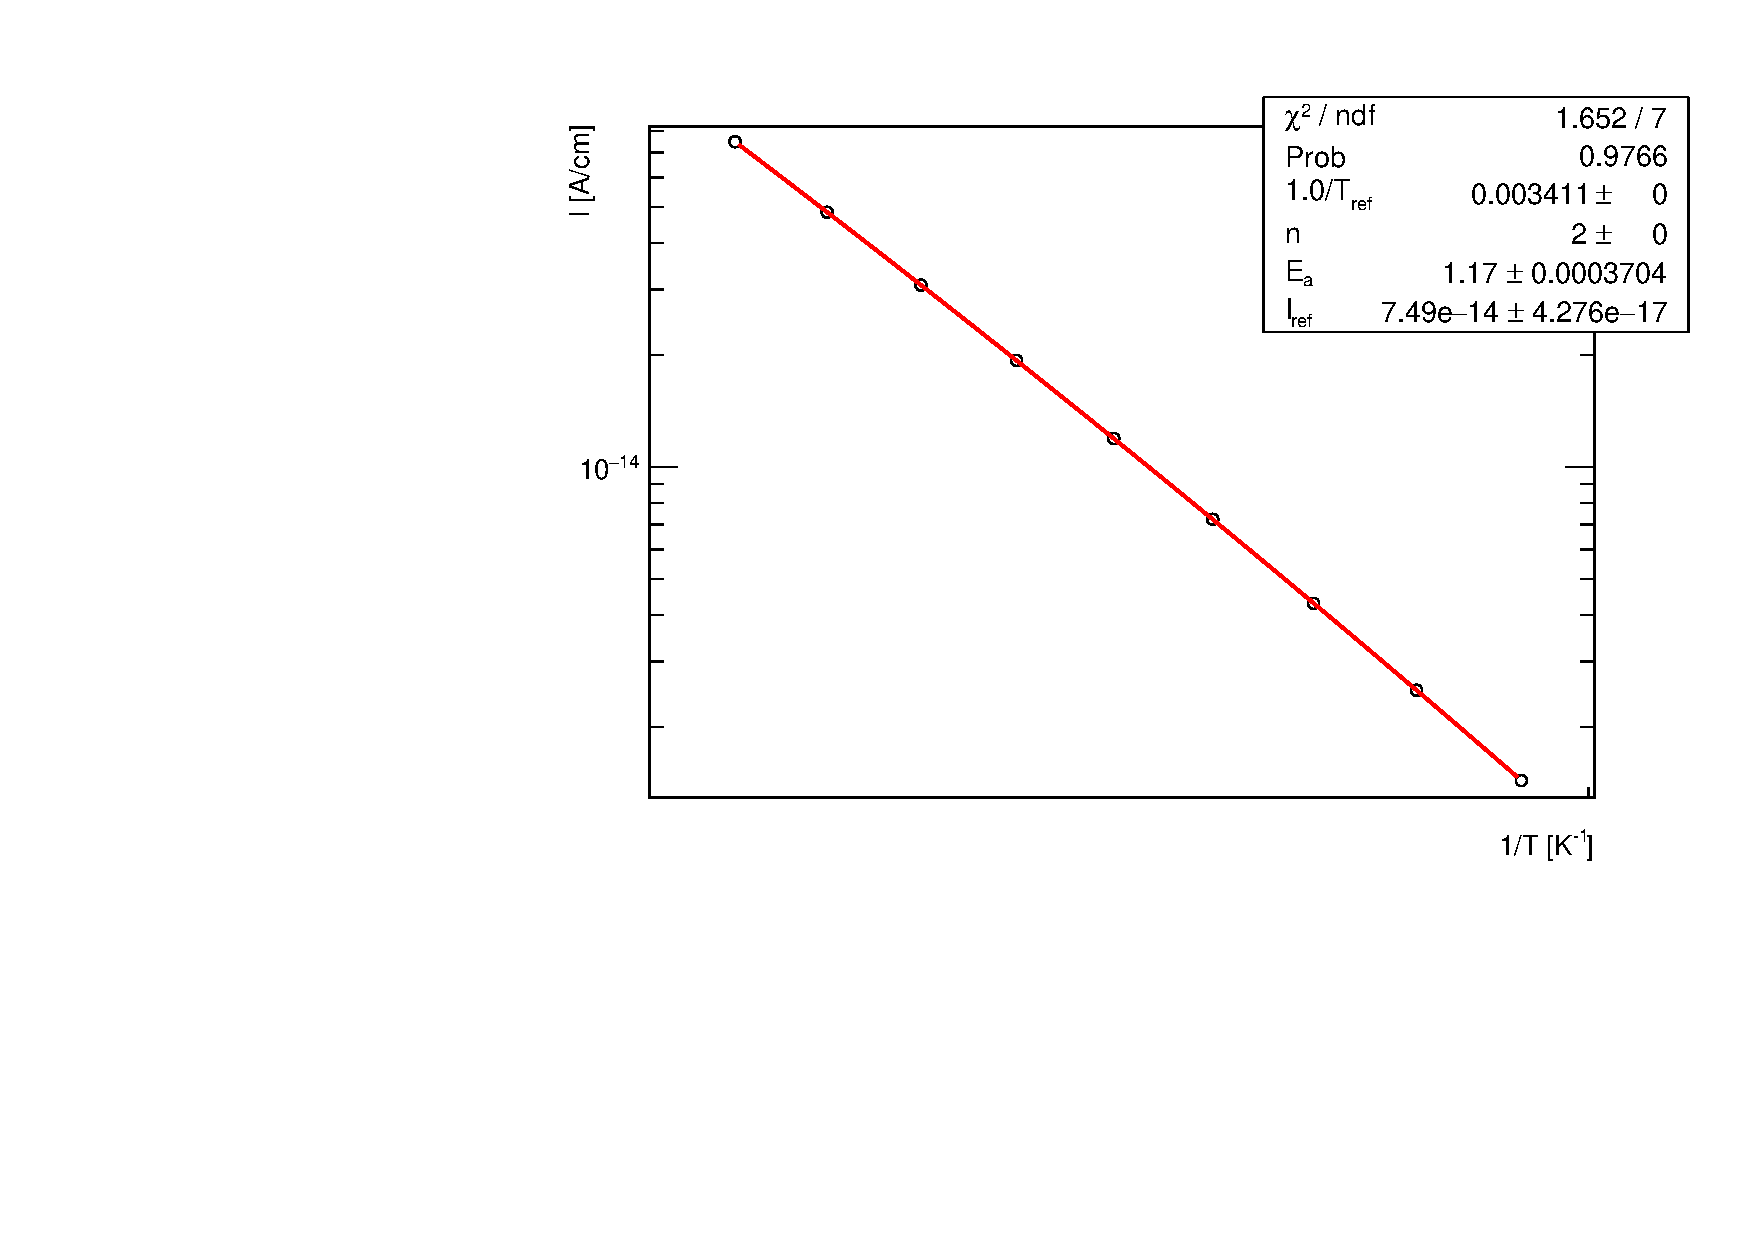
\includegraphics[width=0.49\textwidth]{EG112_Syopsys_thermal_velocities/Ea_Fit_fixn.pdf}
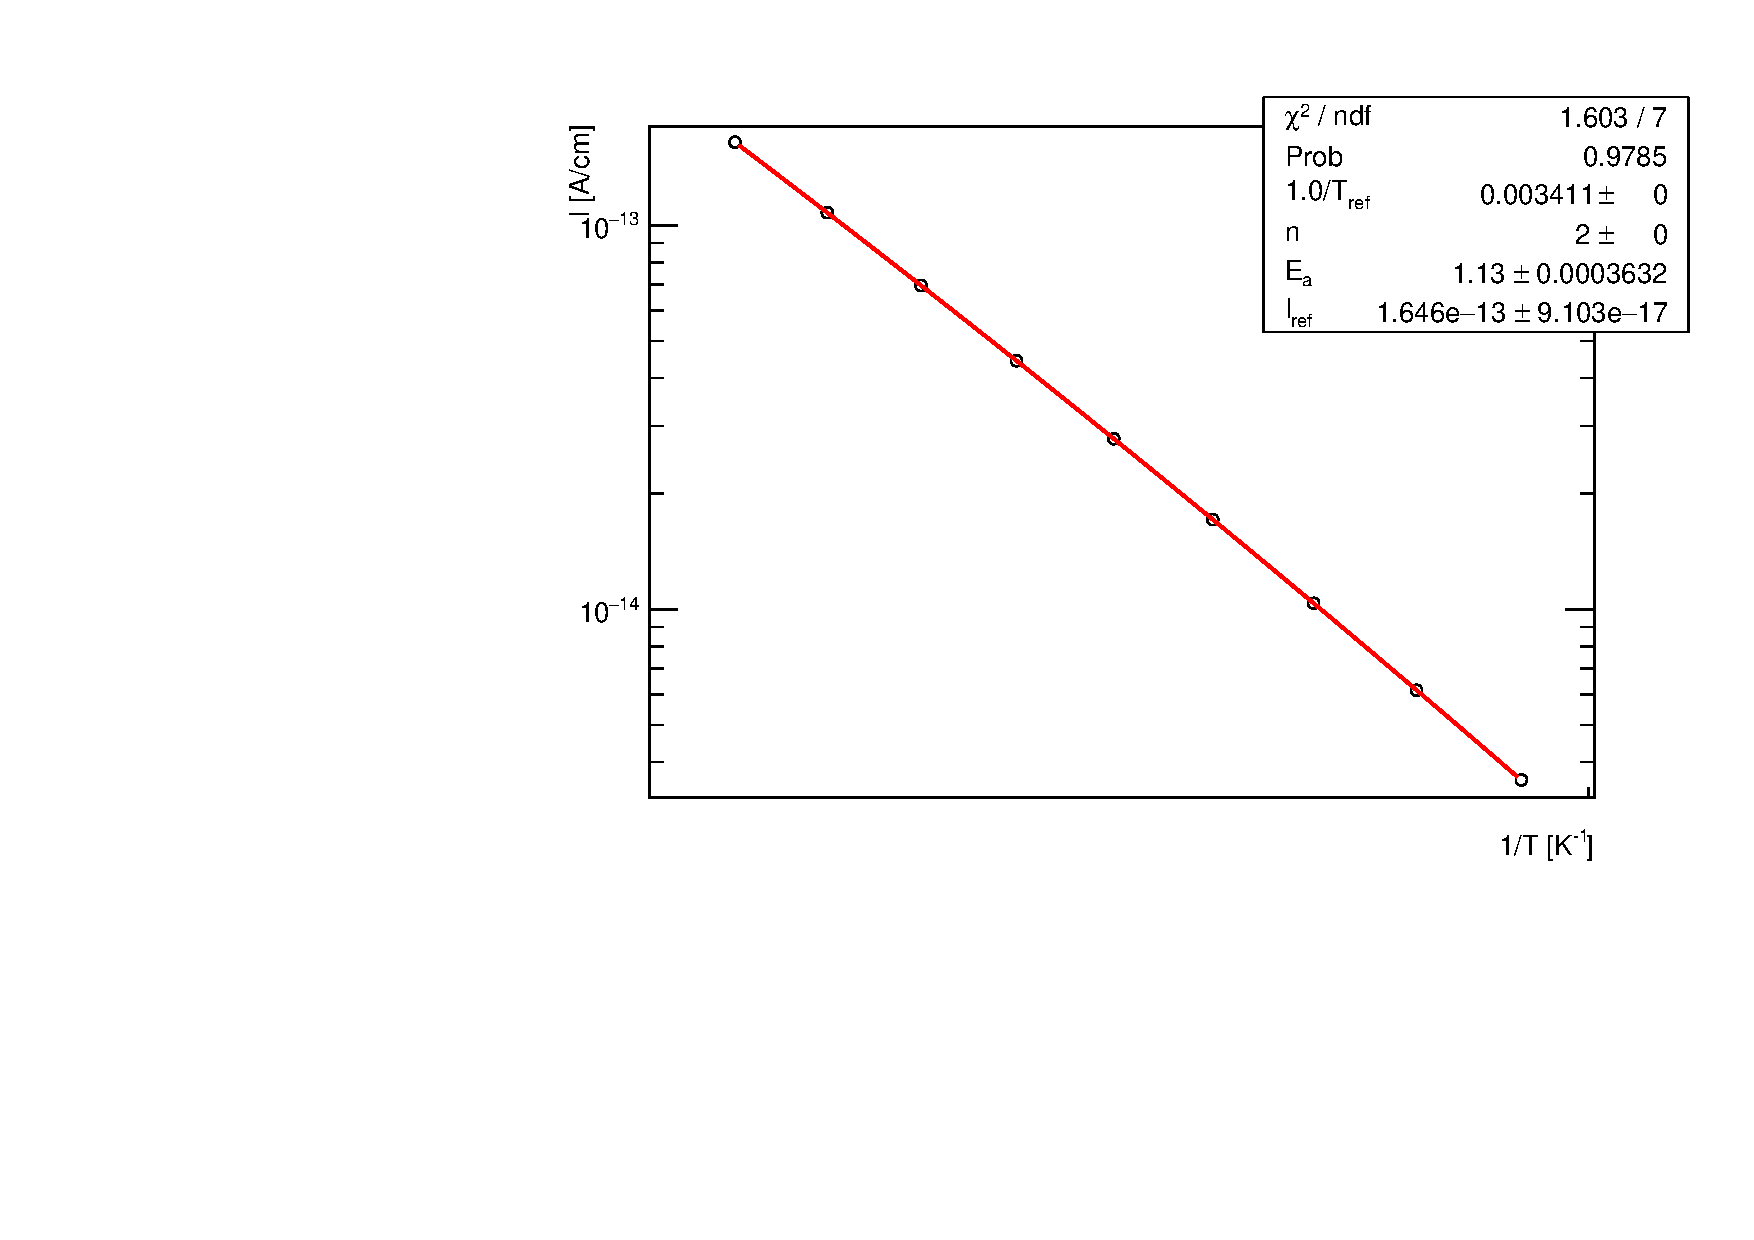
\includegraphics[width=0.49\textwidth]{nobgn/Ea_Fit_fixn.pdf}
\caption{\label{fig:Ea_Fit_fixn}. Simulated leakage current at operational voltage $V_{op}$ at different 
temperatures for different scenarios. (Top row) default scenario; (mid row) EG112 scenario on the left,  Syn. Th. Vel. on the right;  (bottom row)  EG112 \&  Syn. Th. Vel. scenario on the left, NO BGN 
on the right. Data are points with error bars; data were fit with Equation~\ref{eq:ITfunc}  and the fit result is superimposed. The parameter $n$  was fixed to 2.}
\end{figure}

The fit function~\ref{eq:ITfunc} represent very well the data, whatever the scenario and the choice 
made for the parameter $n$ (free to float or fixed to 2). This is an indication that the  
mechanism of temperature scaling is the same for all the configuration explored. The case, 
not presented here, of setting the parameter $\alpha$ of Equation~\ref{eq:EgT} was tested too 
but the results were deviating too largely from Equation~\ref{eq:ITfunc} hence considered 
unphysical. 
\newpage
In all scenarios the parameter $n$, when unconstrained, is compatible with the value of 2. So 
in the rest of the discussion we will consider only the case when $n=2$ (Figure~\ref{fig:Ea_Fit}).
A couple more scenarios where studied ($E^{Sil}_g(300)=1.09$~eV~and~1.11~eV) with the 
goal of studying the dependence of $E_a$ on $E^{Sil}_g(300)$. The result are reported in 
Figure~\ref{fig:Ea_vs_Eg}

\begin{figure}[!htbp]
\centering
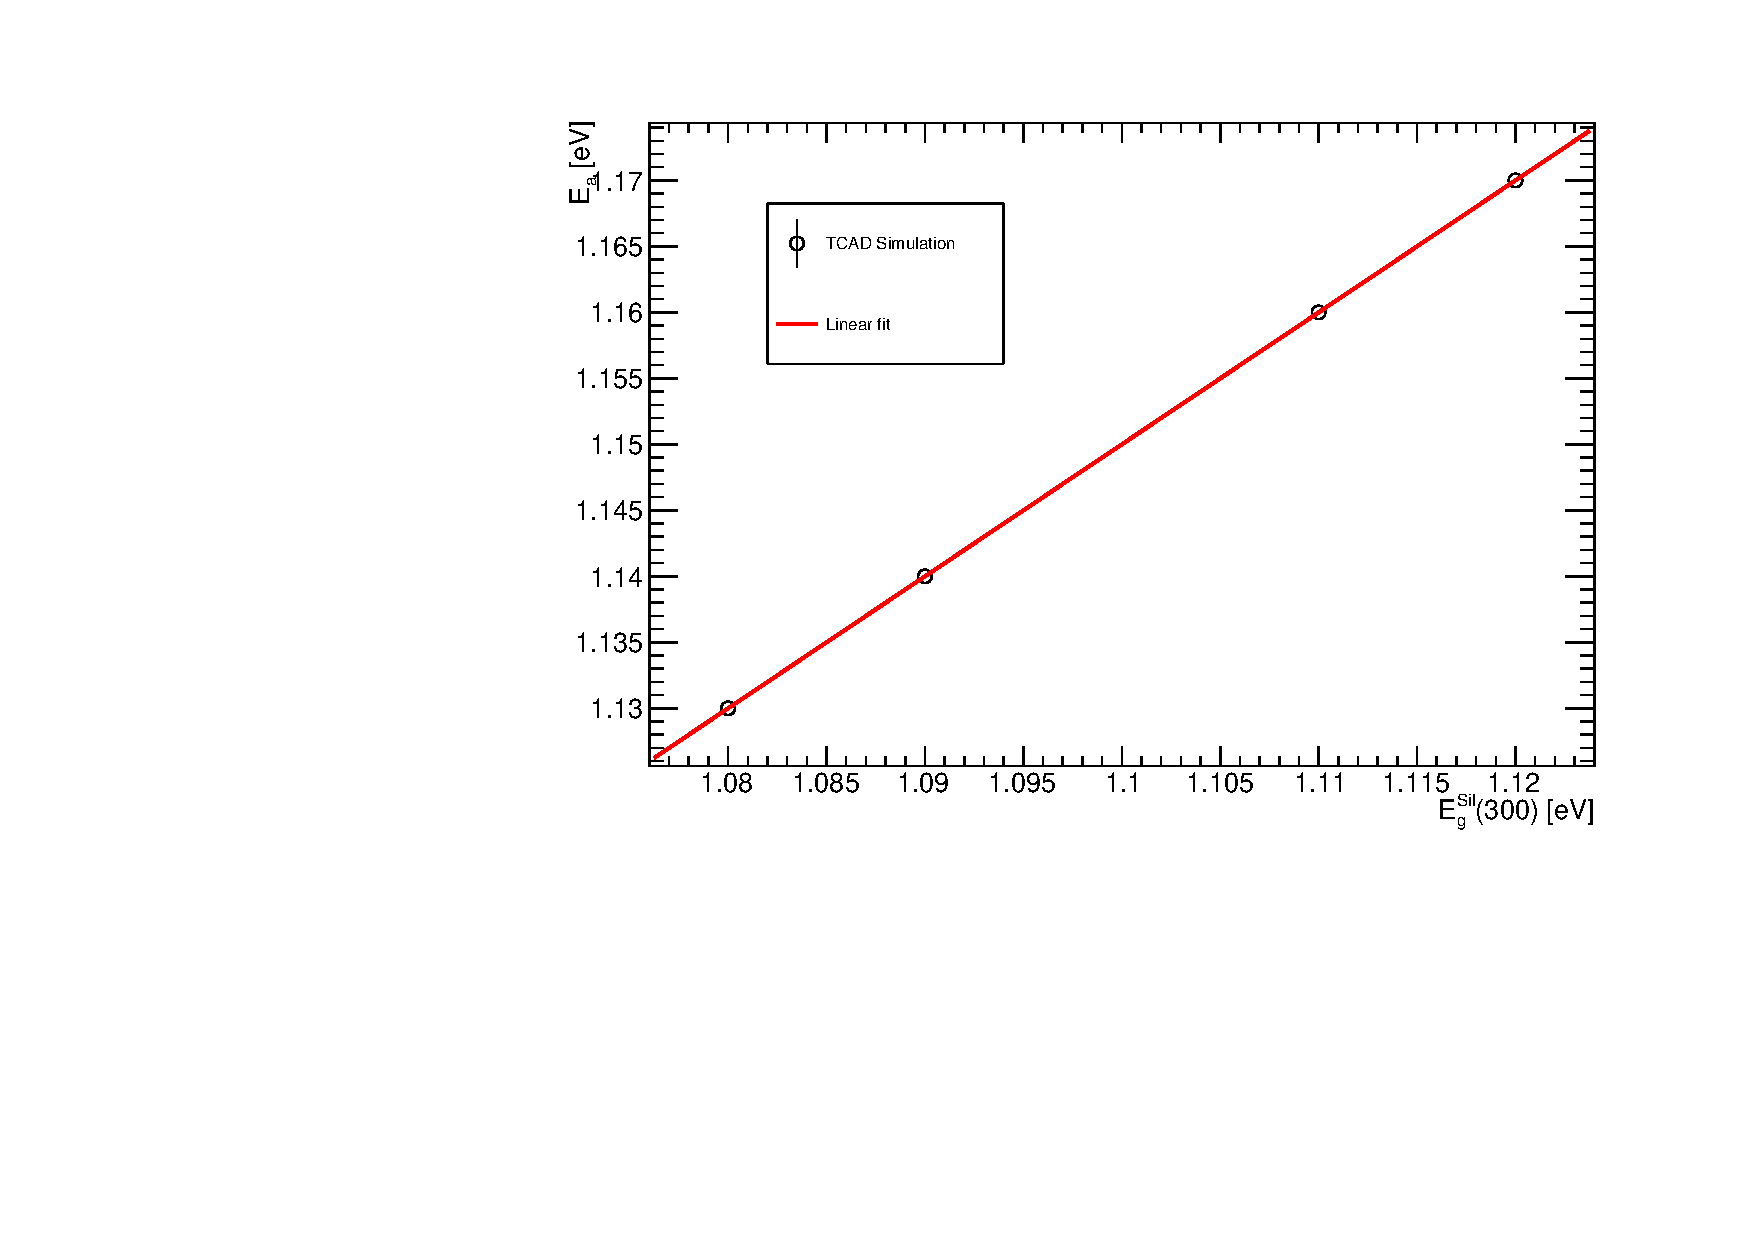
\includegraphics[width=0.65\textwidth]{Ea_vs_Eg.pdf}
\caption{\label{fig:Ea_vs_Eg}Activation energy as a function of the bandgap energy value at 300 K 
in Silvaco TCAD simulation. Data are points with error bars; a linear fit is superimposed.}
\end{figure}
From the Figure is manifest that the following relations hold:

\begin{equation}
E_a=E^{Sil}_g(300)+0.05\,{\rm eV}
\label{eq:Ea_vs_Eg}
\end{equation}

The activation energy range obtained from Equation~\ref{eq:Ea_vs_Eg} does not include 
the value found in literature of 1.21~eV~\cite{Chilingarov_tscale} for bandgap energies between 
1.08~and~1.12~eV.

\subsubsection{Leakage Current Rescaling Based on Temperature}

The relation~\ref{eq:Ea_vs_Eg} was  used with Equation~\ref{eq:IleakT} to rescale 
leakage currents from different temperatures to the reference temperature, $T=293.15$~K 
in this case. The rescaling was done separately for each voltage point. 
 To verify the validity of the rescaling the scaled IV curves 
where divided by the IV curve at the reference temperature. For each 
temperature then the average and the RMS  of these ratio was calculated. 
In Figure~\ref{fig:scaling} the result of this study. It can be seen that after depletion (around -100~V) 
the ratio is very close to 1, much more than in underdepletion. 
If the average values are taken into account then it is possible to estimate to 1\% the accuracy 
on average of the rescaling in the considered temperature range. The slope of the linear fit 
is compatible with 1 as the intercept with 0 within one standard deviation.



\begin{figure}[!htbp]
\centering
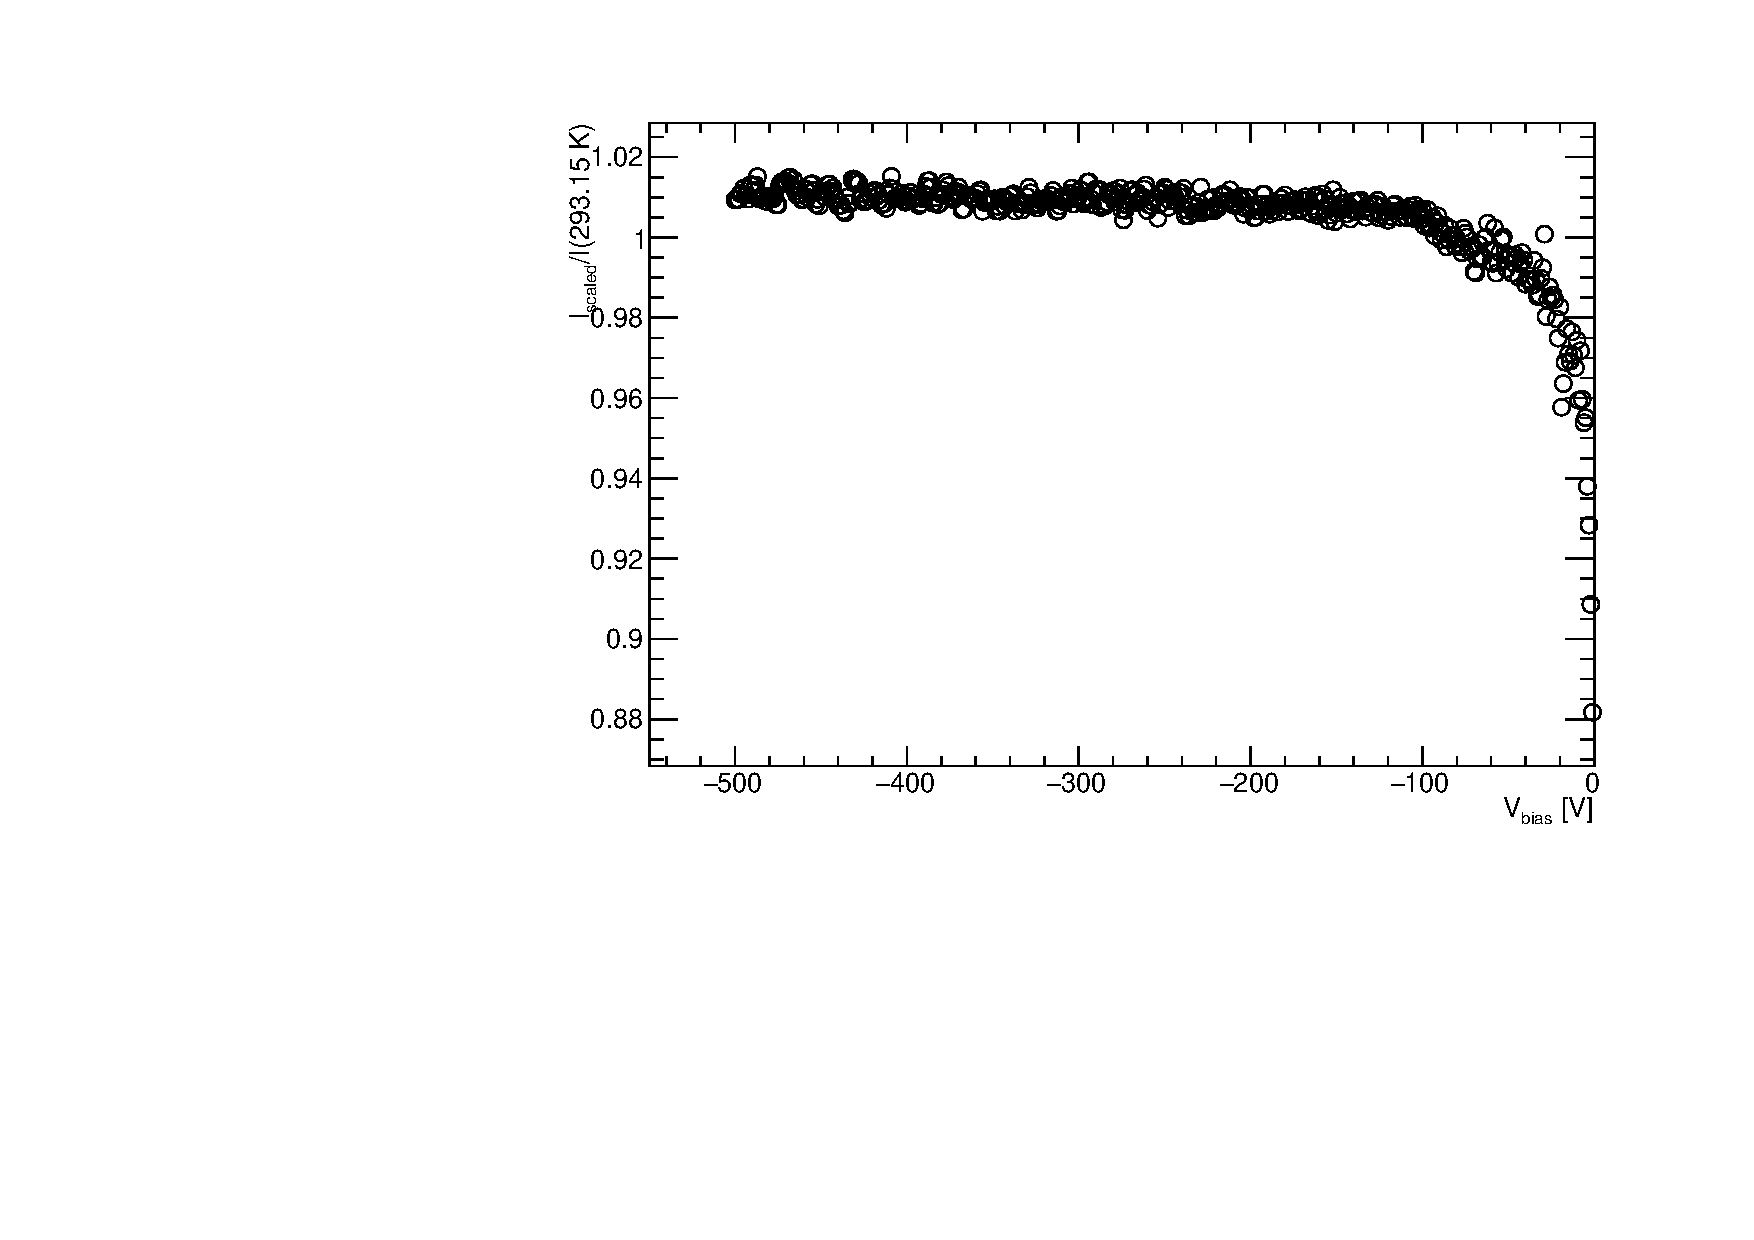
\includegraphics[width=0.49\textwidth]{default/scaled_ratio_T-20.pdf}
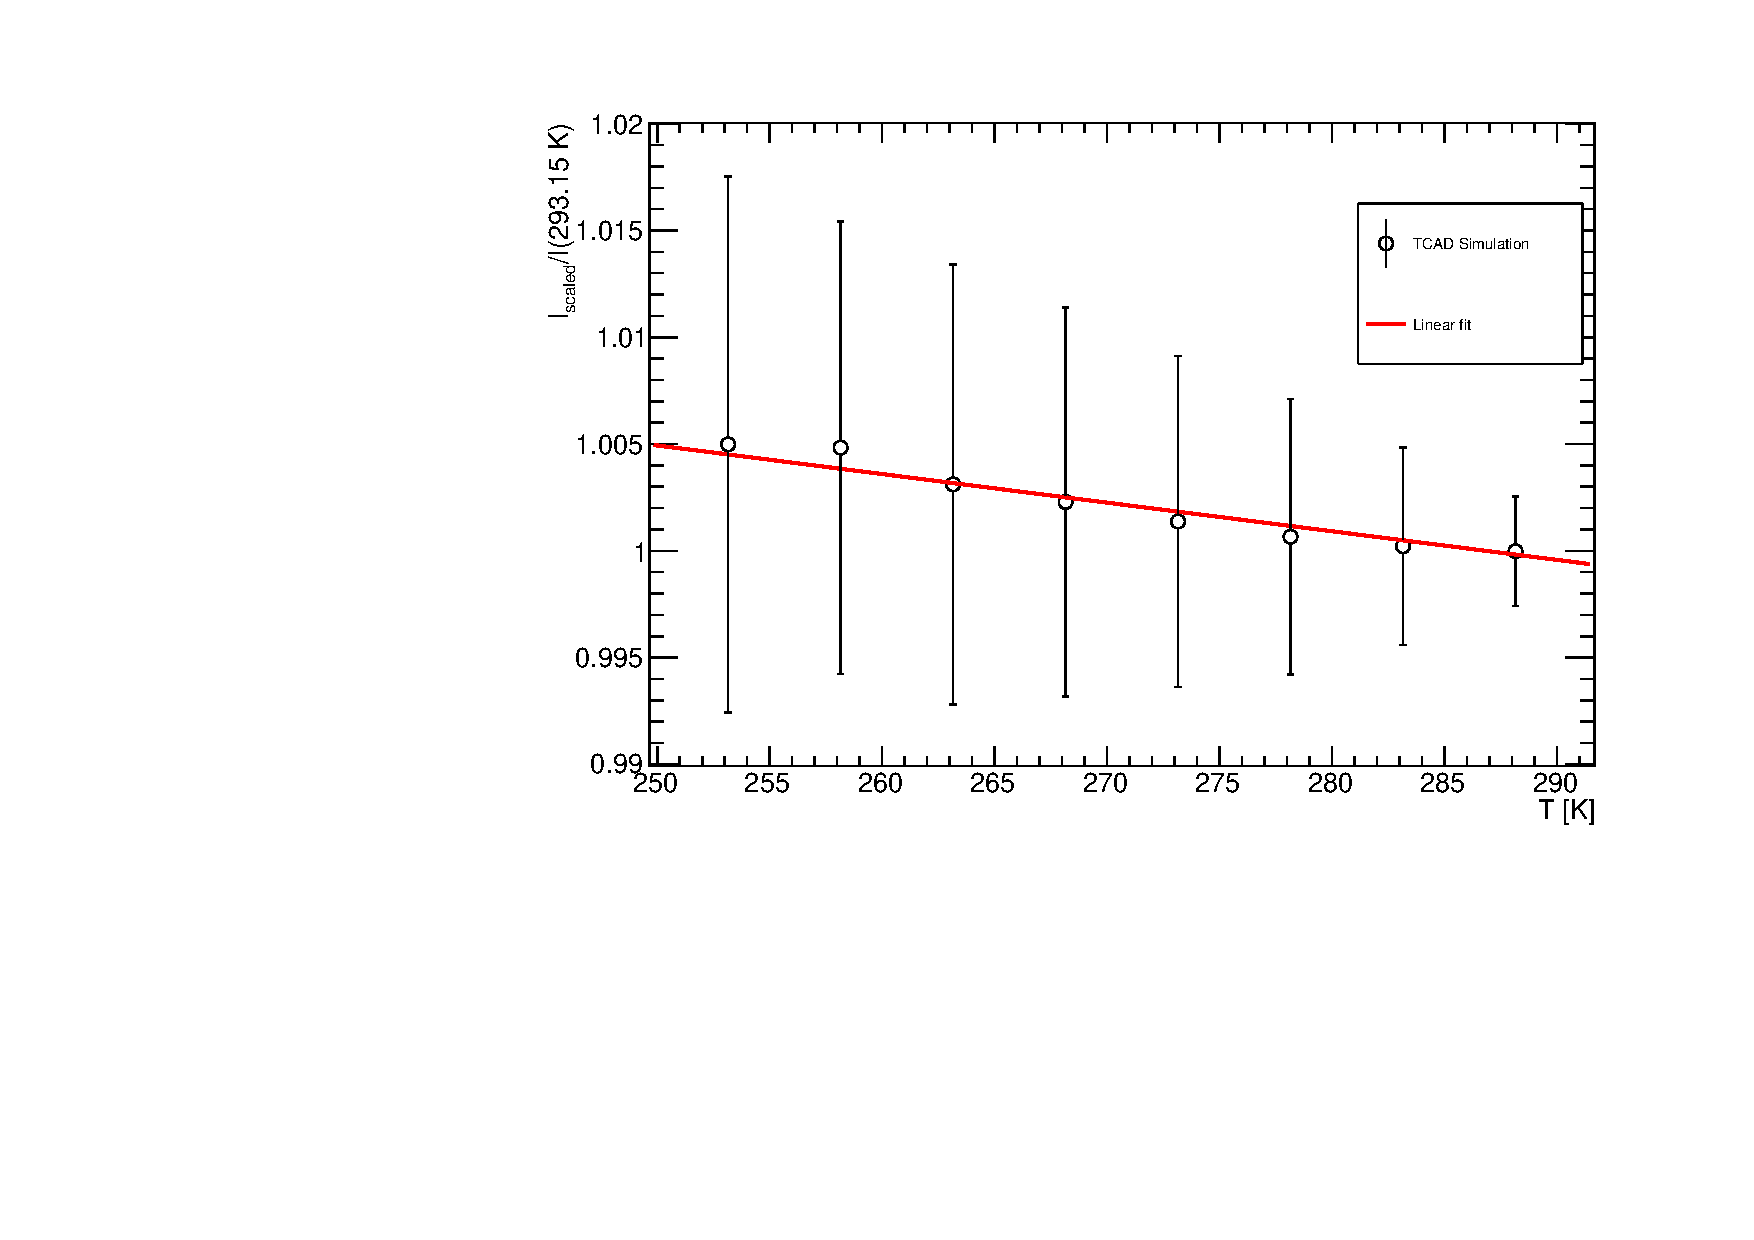
\includegraphics[width=0.49\textwidth]{default/scaling.pdf}
\caption{\label{fig:scaling}.(Left) ratio of IV curve at $t=-20^{\circ}$~C to the one at $t=20^{\circ}$~C 
after the former has been rescaled to $t=20^{\circ}$. (Right) Average ratio of scaled currents to reference one as a function of the temperature. Both plots were created under the default scenario.}
\end{figure}

As  a last test the ratio of IV curve of EG112 scenario to the default one was taken for 
$t=20^{\circ}$C; the curves were taken form~\ref{fig:ILeak20C}. The result is reported in Figure~\ref{fig:EG112_to_default_T_20_Current_ratio}.

\begin{figure}[!htbp]
\centering
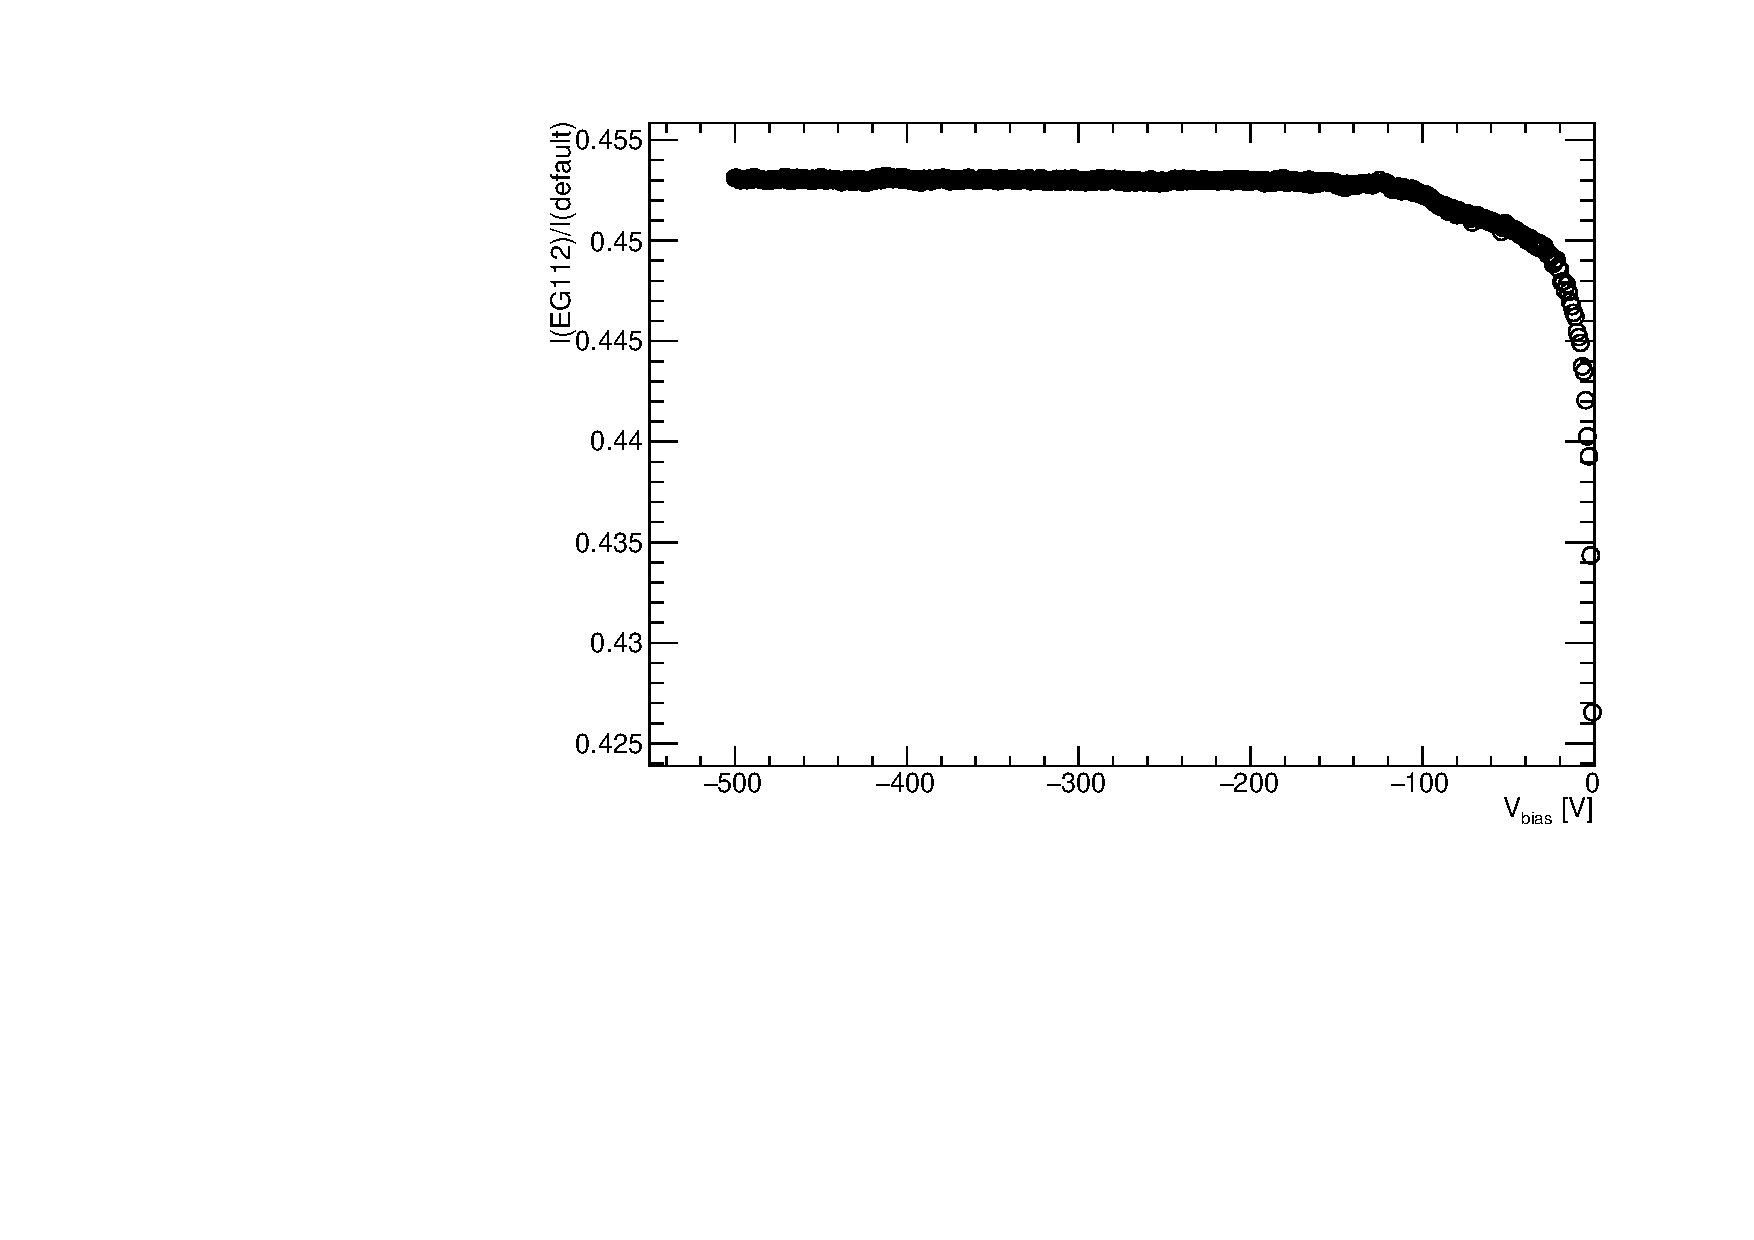
\includegraphics[width=0.65\textwidth]{EG112_to_default_T_20_Current_ratio.pdf}
\caption{\label{fig:EG112_to_default_T_20_Current_ratio}Ratio of IV curve under the EG112 
scenario to the default one. The temperature was $t=20^{\circ}$~C for both scenarios.}
\end{figure}

The average value of the ratio is about 0.4522$\pm$0.0022 which is very close to the theoretical 
prediction based on Equation~\ref{eq:IleakT} used with relation~\ref{eq:Ea_vs_Eg}.


\subsubsection{Summary}
It was shown that there are significant differences between the Synopsys and Silvaco TCAD tools 
on what concerns fundamental parameters like thermal velocities and bandgap energy. 
If for the former a simple rescaling of the carrier effective masses seem sufficient (more in 
the next section), the bandgap energy difference needs a more careful treatment. 

It was shown that, despite the very low default value in Silvaco (1.08~eV at 300~K), the 
simulated leakage current level is in agreement with expectations based on intrinsic concentration 
and generation lifetime when the default value for bandgap energy is considered. TCAD simulated diode reverse leakage currents scale with temperature 
with the same formula which emerged from real data analysis; the fitted value of activation energy 
in simulated data is is very low, though: 1.17~eV maximum with respect to 1.21~eV. 
It was proved that it is possible to effectively rescale the simulated leakage currents from different temperatures to 20$^{\circ}$~C as it is done for real data, once the appropriate activation energy 
value for simulations is used.

In conclusion it seems possible to use TCAD Silvaco tools to perform reliable simulation studies 
on Silicon detectors using the default parameters values, even if they appear to differ significantly 
from the measured ones. 


\section{Modelling Radiation Damage in TCAD Simulations}
\label{sec:TCADRadDamage}

In this Section the implementation, modelling and a  study case of Radiation Damage in TCAD 
Simulations will be presented. This Section is an introduction to a subject that will be 
discussed more in detail later, in Chapters~\ref{chap:ATLAS}~and~\ref{chap:ITk}.

\subsection{Implementation of Radiation Damage in TCAD Simulations}
As it was discussed in Section~\ref{sec:RadDam} energetic particles above a certain energy threshold 
create defects called Frenkel pairs. 
It is possible to simulate defects using TCAD tools by adding trap centers, or simply {\it traps}, to the 
energy bandgap. 
Trap centers, whose associated energy lies in a forbidden gap, exchange charge with the conduction 
and valence bands through the emission and capture of electrons. The trap centers influence the 
density of space charge in semiconductor bulk and the recombination statistics.
Device physics has established the existence of three different mechanisms, which add to the space 
charge term in Poissons?s equation in addition to the ionized donor and acceptor impurities. These are 
interface fixed charge, interface trap states and bulk trap states. Here only bulk traps 
will be discussed. In particular this Section will describe the definition of bulk trap states and the implementation of these bulk trap states into Silvaco TCAD device simulations\footnote{\url{https://www.silvaco.com/products/tcad/device_simulation/atlas/atlas.html}}.

A donor-type trap can be either positive or neutral like a donor dopant. An acceptor-type trap can be 
either negative or neutral like an acceptor dopant. A donor-like trap is positively charged (ionized) when 
empty and neutral when filled (with an electron). An empty donor- type trap, which is positive, can 
capture an electron or emit a hole. A filled donor-type trap, which is neutral, can emit an electron or 
capture a hole. An acceptor-like trap is neutral when empty and negatively charged (ionized) when filled 
(with an electron). A filled acceptor-like trap can emit an electron or capture a hole. An empty acceptor-
like trap can capture an electron or emit a hole. 

Figure~\ref{fig:TCAD_Defects} shows the terminology used within Silvaco TCAD to define the type of trap. The position of the trap is defined relative to the conduction or valence bands using $E.LEVEL$ so for instance, an acceptor trap at 0.4eV would be 0.4eV below the conduction band~\cite{SilvacoAtlas}.

\begin{figure}
\centering
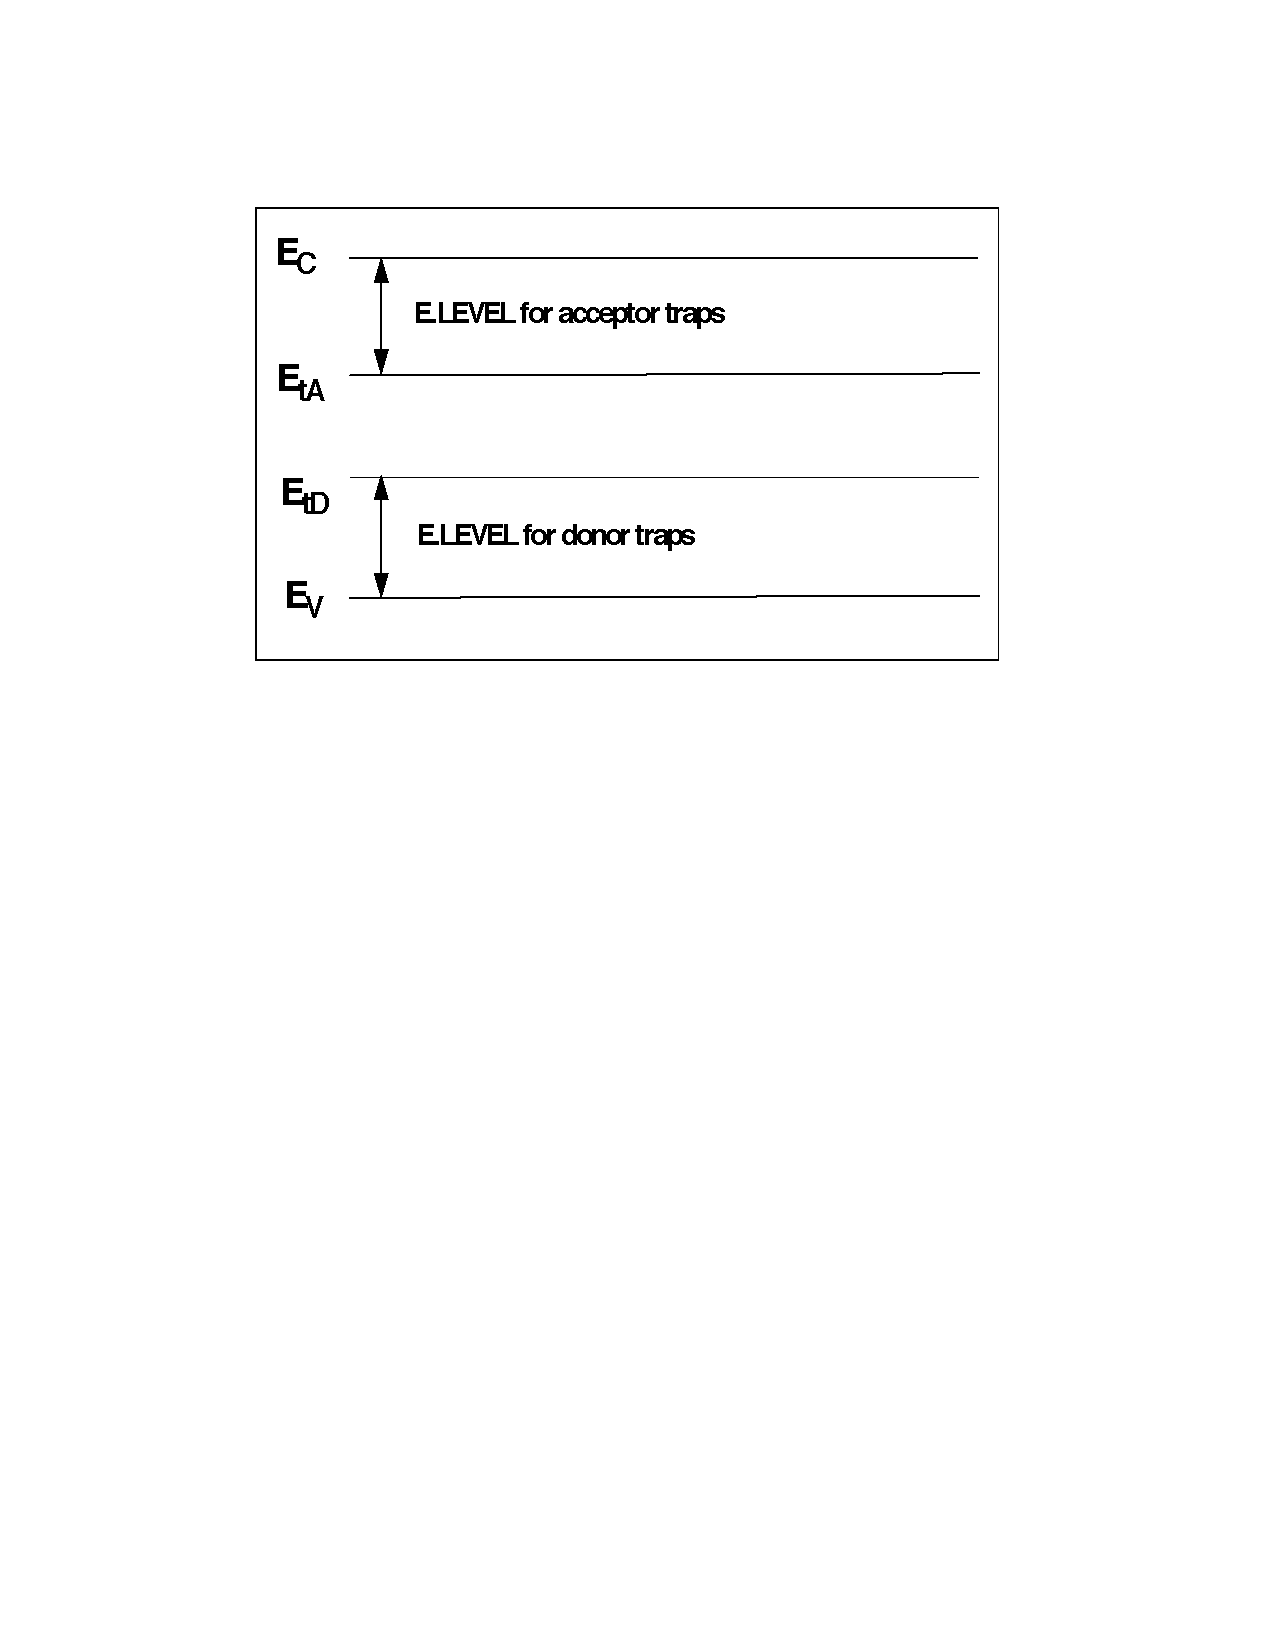
\includegraphics[width=0.65\textwidth]{TCAD_traps.pdf}
\caption{\label{fig:TCAD_Defects}Definition of the trap energy level for acceptor and donor traps in reference to thec onduction and valence band edges. (After~\cite{SilvacoAtlas})}
\end{figure}

The total charge caused by the presence of traps is added to the right side of the Poisson Equation; 
the generation-recombination equations will be modified including terms for talking into account 
that electrons are being emitted or captured by the donor and acceptor-like traps.



\subsection{Radiation Damage Modelling in TCAD Simulations}

We will now discuss which traps are to be added to TCAD Simulations to reproduce the 
experimental observations presented in~\ref{sec:RadDam}.
A list of defects relevant for silicon diode used in HEP was shown 
in Figure~\ref{fig:Defects}.  Including all these defects is presently infeasible  due to the overwhelming computational effort required and the large uncertainties associated with some levels. 

Simplified approaches are therefore applied where only a subset of defects are simulated~\cite{Passeri1998,Passeri2001,Moscatelli-2002,bib:DP,Moscatelli-2004,Chiochia2005,CHIOCHIA2006,Moscatelli-2006,Pennicard:2008zz,dalal2014simulation,Passeri2015}. 
Historically a simple model which accounts for the bulk damage just by means of one ``equivalent'' 
deep acceptor-like level was tried~\cite{Passeri1998,Passeri2001} but it was failing at reproducing the 
double peak effect in the electric field distribution of heavily irradiated devices as shown in~\cite{Li1992}.
Two traps, one acceptor-like and one donor-like are more suited for this; several models where 
proposed, like~\cite{bib:DP,Chiochia2005,CHIOCHIA2006,dalal2014simulation}. 
Further development involved the introduction of a second acceptor-like trap, very close to the midgap; 
this helped to better model the type inversion and the leakage current increase with 
fluence~\cite{Moscatelli-2004,Moscatelli-2006,Pennicard:2008zz,Passeri2015}. At some point also 
4 traps were considered but this was kind of unique trial~\cite{Moscatelli-2002}.

An example of radiation damage model for TCAD simulations in given in Table~\ref{tab:raddammodelpars}; the traps characteristics are taken from~\cite{Pennicard:2008zz}.

\begin{table}[!htbp]
\centering
\caption{\label{tab:raddammodelpars}Relevant parameters for  acceptors (A) and donor (D) deep levels in the bandgap, describing the radiation damage. (After~\cite{Pennicard:2008zz})}
\begin{tabular}{ccccc}
  Type & Energy (eV) & $\sigma_e (\rm{cm}^2)$ & $\sigma_h (\rm{cm}^2)$ & $\eta  (\rm{cm}^{-1})$ \\ 
  \hline
  A &   $E_C $ -0.42 &  $9.5 \times10^{-15} $ &  $9.5 \times 10^{-14} $ & 1.613 \\
  A &   $E_C $ -0.46  &  $5.0 \times10^{-15} $ &  $5.0 \times 10^{-14} $ & 0.9 \\
  D &   $E_V $ +0.36  &  $3.23 \times10^{-13} $ &  $3.23 \times 10^{-14} $ & 0.9 
\end{tabular}
\end{table}
For each trap it is specified if it is a donor- or an acceptor-like trap, its energy with respect to 
the relevant band edge (conduction / valence for an acceptor-/donor-like trap), the capture 
cross sections~$\sigma_{e,h}$ for electrons and holes, respectively, and the introduction rate $\eta$ 
which is the density of traps $N_t$ per unit of fluence $\Phi$.

In general the energy of the trap $E_t$ is located some units of thermal energy $k_B T$ away from the 
intrinsic energy level $E_i$, the introduction rate $\eta$ is close to unity and the 
capture cross sections $\sigma$ are included in the range $10^{-16}-10^{13}$~cm$^2$.

\subsection{Radiation Damage in TCAD Simulations Case studies}

After the short review of radiation damage models for TCAD Simulations available in literature 
we now discuss briefly how to chose among them.
The choice of the radiation damage model depends of course 
on the level of agreement with real data from irradiated detectors, but there is not a single model 
that can fit all possible real data. This is particularly evident when the electric field profile inside 
the irradiated device is investigated. 

Combining beam test data with TCAD simulations in what is called the {\it grazing angle} 
technique~\cite{Henrich:687041,Lari:2001qqa}  
it is possible to extract the electric field profile along the bulk depth of the irradiated detector.
An example of such studies can be found in~\cite{Chiochia2005,CHIOCHIA2006}; the 
authors investigated $n-on-n$ pixel detectors irradiated at CERN with  24~GeV/c protons. 
The authors measured charge collection profiles as in Figure~\ref{fig:chiochia2006_profiles}. 

\begin{figure}[!htpb]
\centering
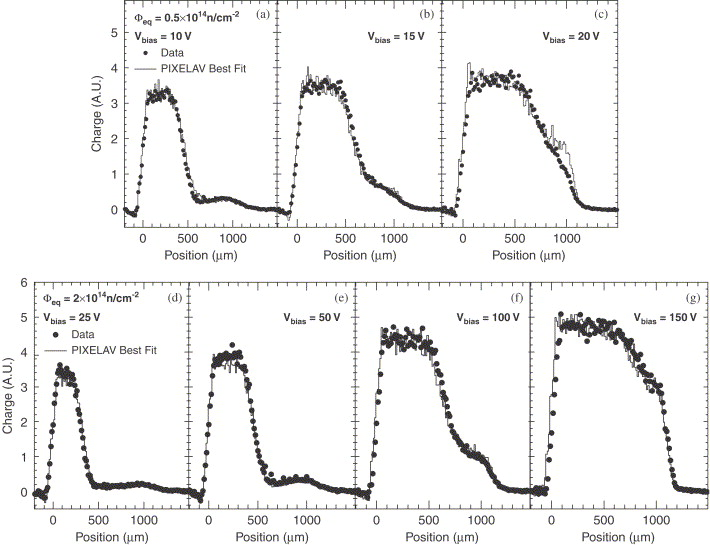
\includegraphics[width=1.00\textwidth]{chiochia2006_profiles.jpg}
\caption{\label{fig:chiochia2006_profiles}Measured (full dots) and simulated (histogram) charge collection profiles for a sensor irradiated to a fluence of $\Phi = 0.5\times10^{14}$~n$_{\rm eq}$/cm$^2$  (a-c) and of $\Phi = 2.0\times10^{14}$~n$_{\rm eq}$/cm$^2$  (d-g), and operated at several bias voltages. (After~\cite{CHIOCHIA2006})}
\end{figure}

To model the local maxima around position~1000~$\mu$m a double peak distribution of  the electric 
field is necessary; they show that a uniform space charge distribution cannot reproduce the 
measured charge profile. 
They propose a radiation damage model based on the work of~\cite{bib:DP}, adapting the 
capture cross sections $\sigma$ and the traps introduction rate $\eta$. Their predictions for the electric field distribution 
are shown in Figure~\ref{fig:chiochia2006_field_profiles}.


\begin{figure}[!htpb]
\centering
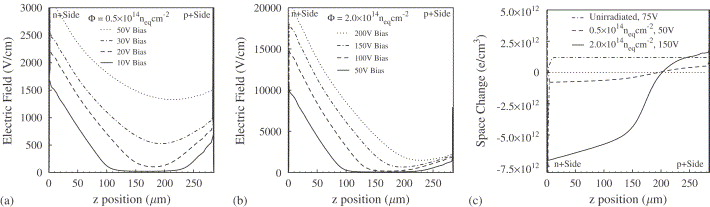
\includegraphics[width=1.00\textwidth]{chiochia2006_field_profiles.jpg}
\caption{\label{fig:chiochia2006_field_profiles}The $z$-component of the simulated electric field  is shown as a function of $z$ for a sensor irradiated to a fluence of  $\Phi = 0.5\times10^{14}$~n$_{\rm eq}$/cm$^2$  (a) and of $\Phi = 2.0\times10^{14}$~n$_{\rm eq}$/cm$^2$  (b).  (c) Space charge density as a function of the $z$ coordinate for different fluences and bias voltages. (After~\cite{CHIOCHIA2006})}
\end{figure}

Recent works~\cite{Macchiolo:2016xzi} that exploited the same technique with 
$n-on-p$ 200~$\mu$m pixel modules irradiated to a fluence of 
$\Phi = 2.0\times10^{15}$~n$_{\rm eq}$/cm$^2$ with 23~MeV protons at 
KIT\footnote{\url{http://www.etp.kit.edu/english/irradiation_center.php}} reported a charge collection 
profile more flat. 

A comparison with TCAD simulations was performed and presented in~\cite{bomben_rd50_Santander}. 
Several models were tried and the best agreement was found when the Perugia 2006 model~\cite{Moscatelli-2006} was used.
\begin{figure}[!htpb]
\centering
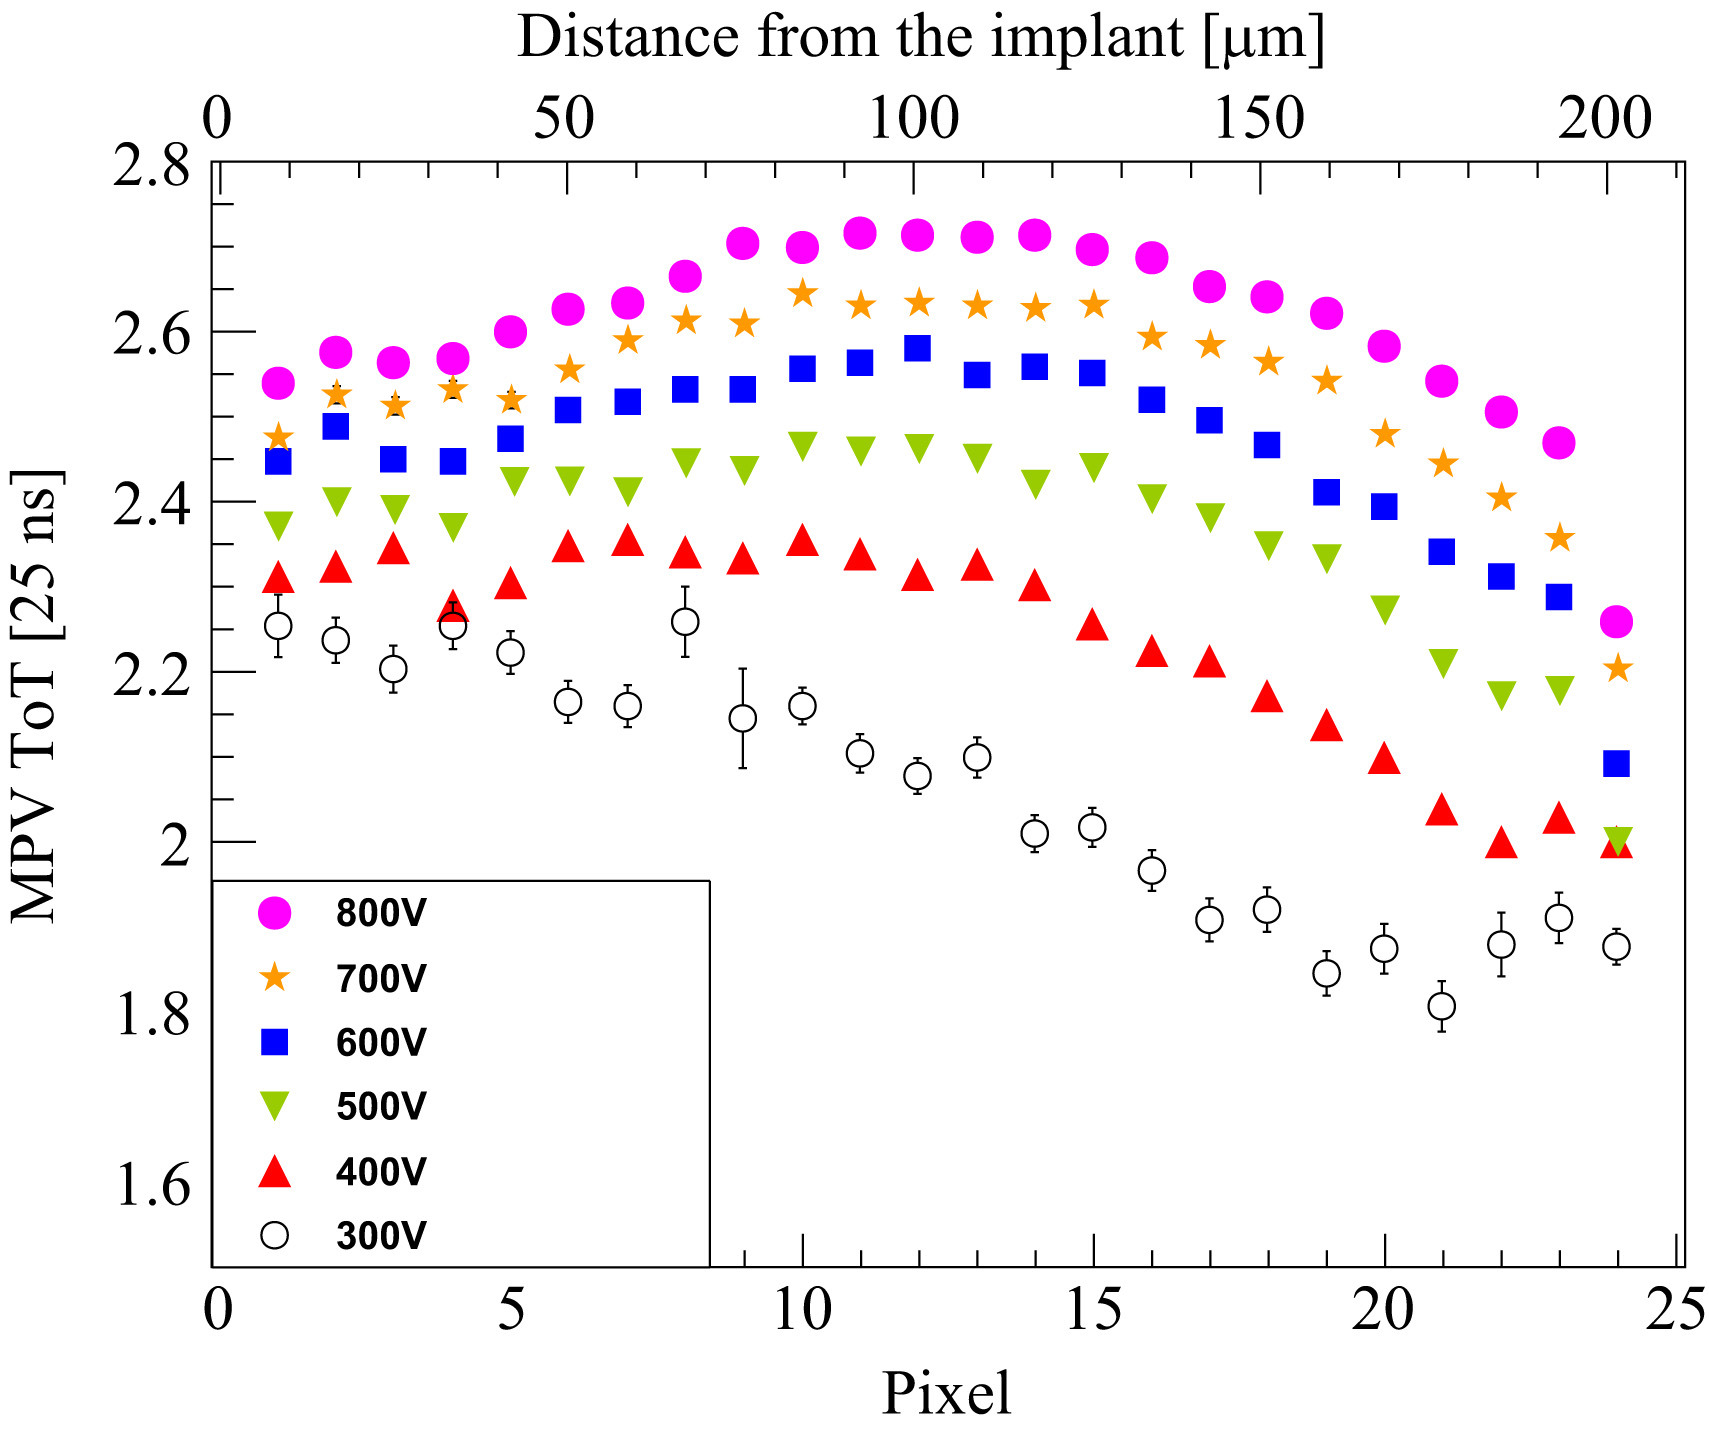
\includegraphics[width=0.39\textwidth]{Savic_high_phi.jpg}
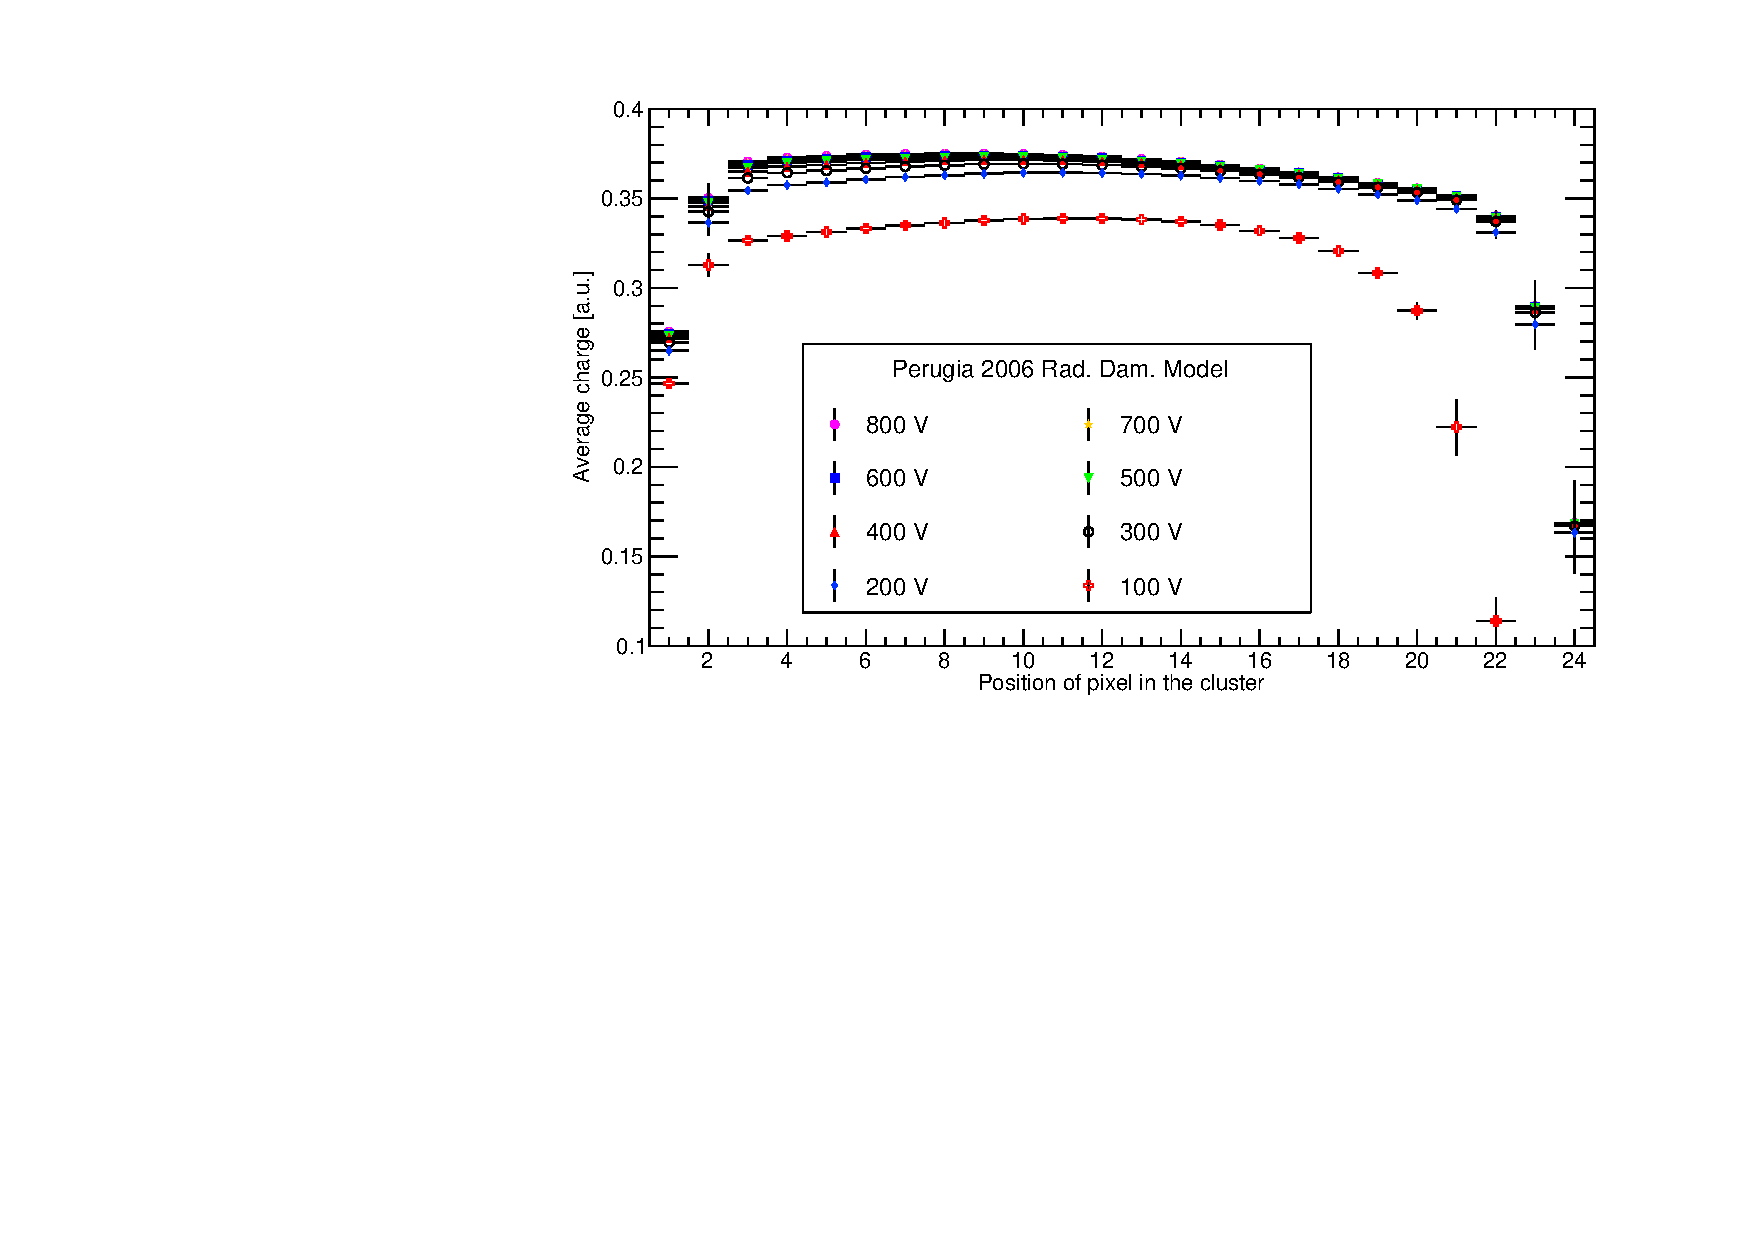
\includegraphics[width=0.59\textwidth]{Pixel_Profile_Perugia2006.pdf}
\caption{\label{fig:Pixel_Profile_Perugia2006}Comparison between (left) measured and (right) 
simulated charge collection profiles for $n-on-p$ 200~$\mu$m thick  pixel modules irradiated to a fluence of 
$\Phi = 2.0\times10^{15}$~n$_{\rm eq}$/cm$^2$. Tracks were impinging at 80$^{\circ}$ with 
respect to detector surface. (After~\cite{Macchiolo:2016xzi,bomben_rd50_Santander})}
\end{figure}
The agreement is qualitative but no other model gave better agreement. In particular models 
predicting a double peak distribution of the electric field where producing charge collection profiles 
more close to the ones presented in Figure~\ref{fig:chiochia2006_profiles} rather the one 
reported here. 

The prediction for the electric field profile from the Perugia 2006 model is presented in 
Figure~\ref{fig:EField_Profile_Perugia2006}.

\begin{figure}[!htpb]
\centering
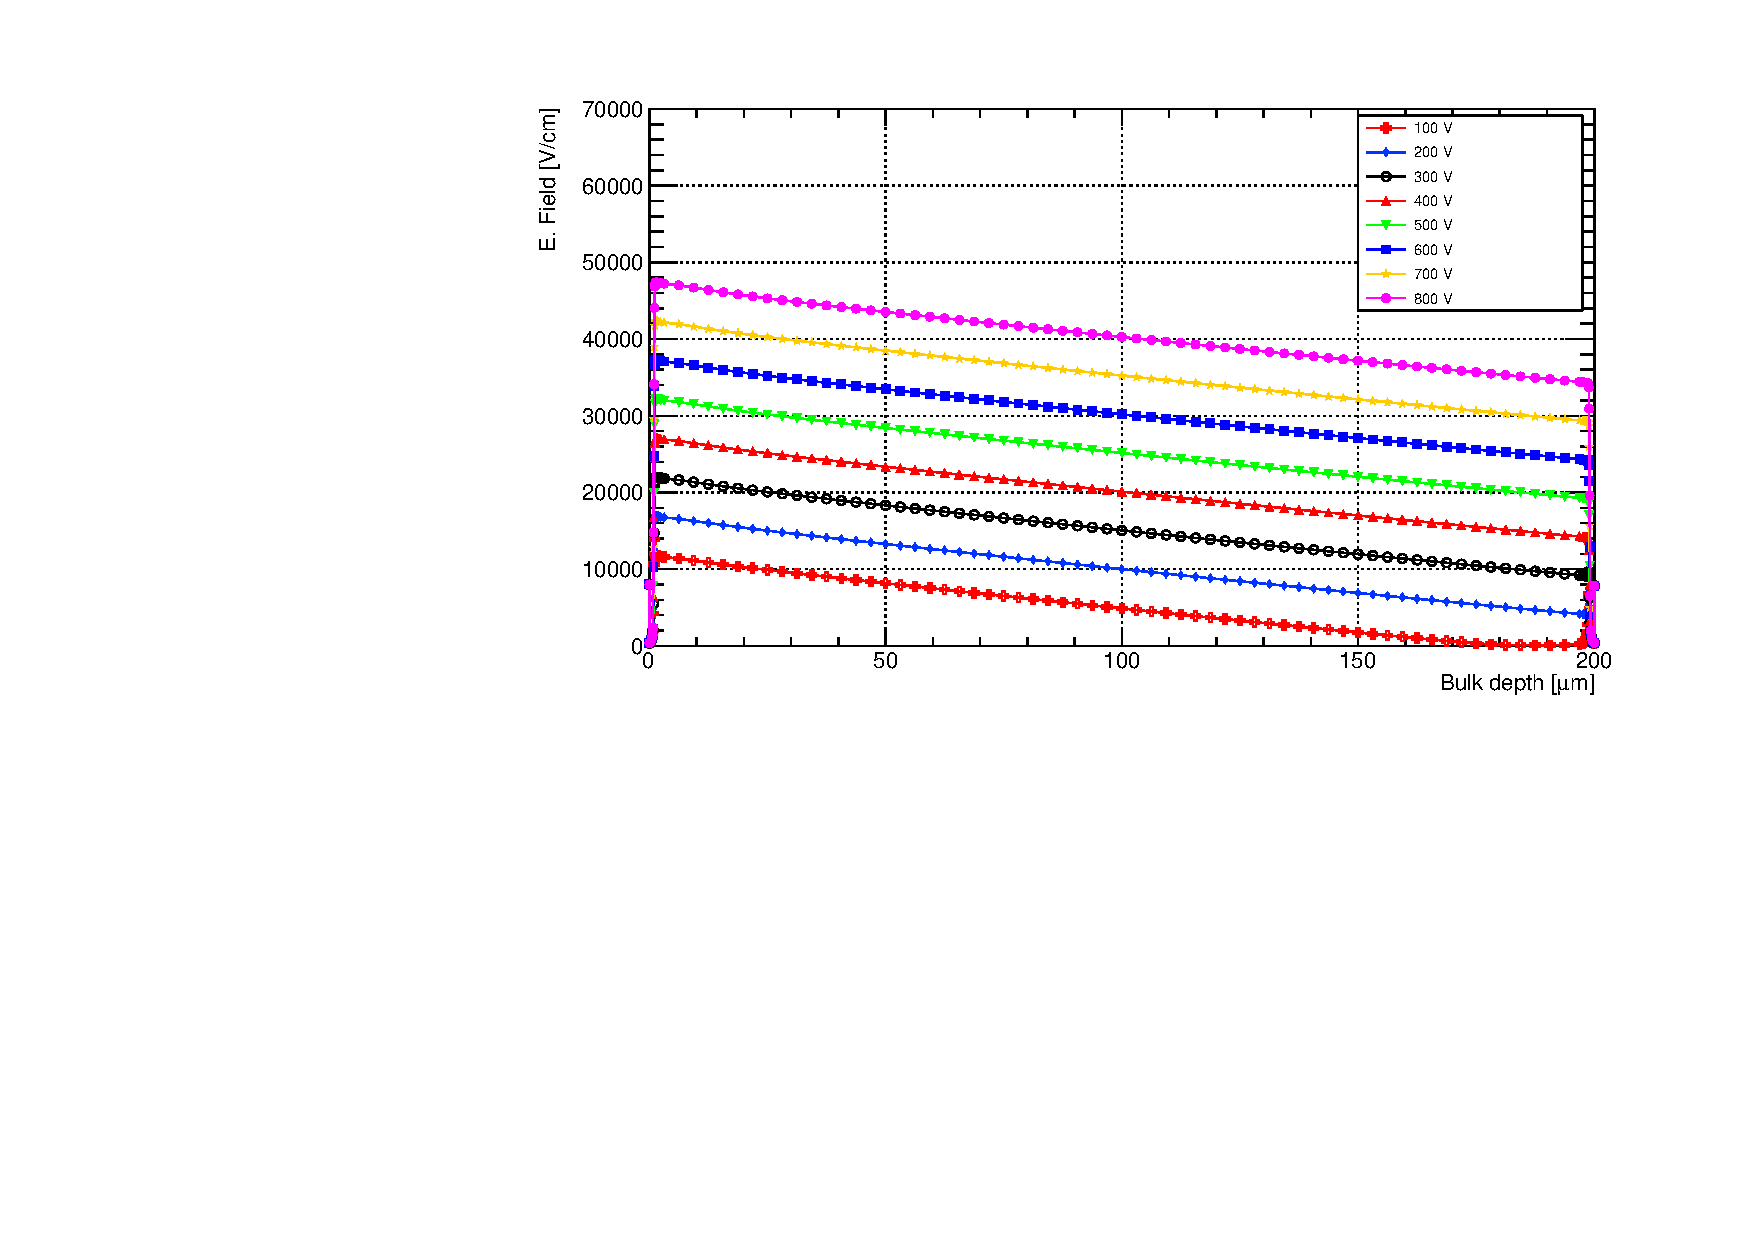
\includegraphics[width=0.65\textwidth]{EField_Natascha_fl2e15_Petasecca.pdf}
\caption{\label{fig:EField_Profile_Perugia2006}Simulated electric field profile for an $n-on-p$ 200~$\mu$m thick pixel modules irradiated to a fluence of 
$\Phi = 2.0\times10^{15}$~n$_{\rm eq}$/cm$^2$. The radiation damage model used was~Perugia 2006\cite{Moscatelli-2006}.}
\end{figure}
As it can be seen the simulated electric field is depending linearly on the bulk depth position, 
as it happens before irradiation. 



\section{Summary}
\label{sec:TCADSummary}

In this Chapter the basics of TCAD simulation of silicon detectors for HEP were presented. 
The motivations for such simulations were discussed and some examples outlined. 
It was shown that, despite some inconsistencies on measured fundamental parameters, TCAD 
simulations can be used to get reliable predictions. 

The interest of using TCAD simulations together with beam test data from heavily irradiated detectors 
was discussed. The issue of the proper choice of radiation damage models for TCAD simulations 
was briefly mentioned; it will be discussed more in detail in Chapter~\ref{chap:ITk}. 
In Appendix~\ref{sec:TCADComparison} a detailed discussion on comparing Silvaco and Synopsys 
TCAD tools when used for radiation damage modelling will be given.


